\documentclass{pfc}
\usepackage{amsmath}
\usepackage{amssymb}
\usepackage{amsfonts}
\usepackage{mathtools}
\usepackage{pdfpages}
\usepackage{subcaption}
\usepackage{gnuplot-lua-tikz}
\usepackage{pstricks}

\subtitle{Informe final}

\newcommand{\TODO}[1]{{\color{red}\bfseries#1}}
\newcommand{\Nota}[1]{{\color{blue}\itshape#1}}

\newcommand{\CasoUso}[1]{\bigskip%
{\bfseries Caso de uso: #1}\par}
\newcommand{\IncCU}[1]{{\bfseries Include (#1)}}
\newcommand{\UseCU}[1]{{\bfseries Use (#1)}}
\newcommand{\CUField}[2]{{\bfseries#1:} #2\par}
\newcommand{\CUNormal}{{\bfseries Curso Normal:}\par}

\newenvironment{CasoDeUso}[1]{%
	\bigskip\begin{minipage}{.9\linewidth}
		{\bfseries Caso de uso: #1}\par
}
{%
	\end{minipage}
}


\newcommand{\Requerimiento}[2]{%
	\bigskip%
	{\bfseries #1}\\%
	#2%
}

\usepackage{algorithmicx}
\usepackage{algorithm}
\usepackage[noend]{algpseudocode}
\usepackage{booktabs}


\makeatletter
 \renewcommand{\ALG@name}{Algoritmo}
\makeatother
\renewcommand{\algorithmicfunction}{}

%\newcommand{\Alerta}[1]{{\Huge\bfseries\sffamily#1}}
\newcommand{\NombreItem}[1]{{\bfseries#1:}}

\usepackage{tikz}
\usetikzlibrary{arrows,chains,matrix,positioning,scopes}

\usepackage{environ}
\makeatletter
\newsavebox{\measure@tikzpicture}
\NewEnviron{scaletikzpicturetowidth}[1]{%
  \def\tikz@width{#1}%
  \def\tikzscale{1}\begin{lrbox}{\measure@tikzpicture}%
  \BODY
  \end{lrbox}%
  \pgfmathparse{#1/\wd\measure@tikzpicture}%
  \edef\tikzscale{\pgfmathresult}%
  \BODY
}
\makeatother

\newcommand{\bigO}{\mathcal{O}}
\newcommand{\Real}{\mathbb{R}}
\DeclareMathOperator*{\argmin}{argmin}
\DeclareMathOperator{\atan}{atan}

\graphicspath{{./uml/}{./diagram/}{./graph/}}

\newcommand{\RefImagen}[1]{ (Imagen cortesía de \cite{#1})}

\includeonly{resultados_b}
\begin{document}
\frontmatter
%\TODO{revisar tiempos verbales, ahora en pasado}
	\maketitle

	\chapter{Resumen}
Gracias a los avances en sensores de profundidad y técnicas de reconstrucción de superficies,
es posible obtener con gran precisión una nube de puntos que represente
la forma, posición y dimensiones de un objeto cualquiera.
Sin embargo, esta nube de puntos es parcial, ya que solamente refleja
la porción observable desde el punto de captura.
Por esta razón, en este proyecto se propone el desarrollo de una biblioteca de software
que implemente técnicas para combinar estas vistas parciales
y así obtener un modelo tridimensional de todo el objeto,
posibilitando su posterior construcción mediante técnicas de impresión 3D.

\Nota{
	sensores de profundidad y técnicas para determinar la profundidad.

	Hablar de prime-sense, kinect fusion, que requieren que el usuario
	tome las capturas con mucho cuidado

	Nosotros hacemos pocas capturas espaciadas, esa es la gracia
%TODO: motivación continuar lo de pancho
%explayarse en la forma de adquisición
%vistas parciales
}
	%\noindent{\bfseries Palabras clave:} fusión de mallas, imágenes de profundidad, impresión 3D, reconstrucción 3D.


	\tableofcontents
	\listoffigures

\mainmatter
	\include{introducción}
	\include{reconstrucción}
	\chapter{Herramientas}
A continuación se describen las principales herramientas de software
utilizadas en el desarrollo y evaluación de la biblioteca de reconstrucción.

\section{Base de datos}
Uno de los supuestos de este proyecto era contar con un repositorio propio de
mallas tridimensionales.
Para la creación de este repositorio,
se utilizarían los algoritmos de reconstrucción desarrollados en \cite{Pancho},
ubicando al objeto de interés en una base giratoria y realizando capturas
en ángulos espaciados hasta completar una vuelta.
De esta forma, las posiciones de las vistas describirían un círculo centrado en el objeto y
cada captura contendría información de posición ($xyz$) y de textura ($rgb$).
Debido a los tiempos requeridos para calibrar el dispositivo de captura,
este repositorio nunca se materializó,
 por lo que fue necesario buscar otro con características similares.

%\begin{itemize}
%	\item redwood, freibug:
%	rgb y profundidad, pero el movimiento es pequeño y libre
%	(tendría que eliminar intermedios)
%\item middlebury
%	base giratoria, pero sólo RGB
%	(tendría que generar el mapa de profundidad)
%\item stanford
%	base giratoria, nube de puntos, sin textura.
%	Se optó por esta.
%	Se decidió no generar artificialmente los puntos de textura para tener un
%	caso más real.
%\end{itemize}

Se decidió utilizar \emph{The Stanford 3D Scanning Repository}\cite{StanfordScanRep} que brinda
acceso a escaneos tridimensionales y reconstrucciones detalladas para ser
usados en investigación.

Las capturas fueron obtenidas mediante un escáner láser de barrido Cyberware
3030~MS.  Se realizaron escaneos del objeto en diversas posiciones sobre una
base giratoria y luego estas capturas fueron combinadas para producir una única
malla triangular mediante el método de \emph{zippering}\cite{Turk:1994:ZPM:192161.192241} o el de
\emph{volumetric merging}\cite{Curless:1996:VMB:237170.237269}, ambos desarrollados en
Stanford.

La base de datos provee un archivo de configuración con las transformaciones de
alineación requeridas por cada captura.
Estas transformaciones fueron obtenidas realizando la registración de cada captura
contra un escaneo cilíndrico del objeto mediante un método semiautomático, donde el usuario
usuario establece una alineación inicial que luego es ajustada mediante un algoritmo
basado en ICP\cite{Turk:1994:ZPM:192161.192241}.

De esta base de datos se escogieron los modelos
	\texttt{armadillo},
	\texttt{bunny},
	\texttt{dragon},
	\texttt{drill} y
	\texttt{happy},
los cuales presentan distintos niveles de detalles, cantidad de escaneos y niveles de ruido.


\begin{figure}
	\Imagen{img/stanford_models}
	\caption[Modelos de la base de datos Stanford]{\label{fig:stanford_models}Modelos de la base de datos Stanford.
		De izquierda a derecha y de arriba a abajo, los modelos son:
		\texttt{armadillo},
		\texttt{bunny},
		\texttt{dragon},
		\texttt{drill}
		y \texttt{happy}.
		En el caso del modelo \texttt{drill}, sólo se presenta la reconstrucción de la mecha, descartando la estructura de apoyo.}
\end{figure}


Desgraciadamente, no se cuenta con información de color en estos escaneos.
Se decidió adaptar los algoritmos a esta situación, en lugar de agregar
artificialmente valores de color para los puntos.


\section{Tecnologías}
	%Intro
Las siguientes tecnologías fueron consideradas y evaluadas
para el diseño y desarrollo de las funcionalidades de la biblioteca,
si bien algunas debieron ser descartadas por no ajustarse a las restricciones
y supuestos establecidos para el producto.

	\subsection{KinectFusion}
	%algoritmo, incluido en la sdk de kinect v2
	El algoritmo de KinectFusion fue desarrollado por Microsoft
	para lograr reconstrucciones tridimensionales utilizando el dispositivo Kinect.

	%kinectfusion_real-time_3d_reconstruction_and_interaction_using_a_moving_depth_camera
	Debido a que uno de sus objetivos era lograr una implementación en tiempo
	real, el algoritmo de registración requiere de poca variación
	de la posición relativa cámara-objeto entre capturas, por lo que fue descartado.

	La fusión se realiza mediante una variación del método de
	\emph{volumetric merging} sobre GPU\cite{Izadi:2011:KRR:2047196.2047270}.

	%Suposiciones:
	%transforma el sistem en uno lineal, la transformación entre capturas es un incremento pequeño
	%sistema 6x6 (3 translaciones, 3 rotaciones)
	%utiliza todos los puntos porque tiene gpu




	\subsection{Open Source Computer Vision Library (OpenCV)}
	Es una biblioteca de código abierto de visión computacional y aprendizaje
	maquinal.  Cuenta con módulos de procesamiento de imágenes de profundidad y
	registración.

	En un principio se consideró utilizar la información de color de las capturas
	para poder lograr la registración, pero debido a que la base de datos
	finalmente elegida contiene únicamente información geométrica
	no se podrán aprovechar las funcionalidades de esta biblioteca.

	\subsection{\emph{The Point Cloud Library} (PCL)}
	Es un framework de código abierto multiplataforma para el procesado de
	imágenes 2D/3D y nubes de puntos.
	Provee numerosos algoritmos modernos para reducción de ruido, extracción de
	puntos salientes, cálculo de descriptores, registración, reconstrucción de
	superficies, entre otros\cite{5980567}.
	Además, contiene el módulo KinFu, el cual es una implementación libre del algoritmo KinectFusion
	donde se elimina la dependencia con el dispositivo Kinect,
	se presentan algoritmos para trabajar a una mayor escala
	y se permite la integración de la información de textura a la superficie final reconstruida\cite{real-time-3d-reconstruction-using-a-kinect-sensor}.

	La documentación incluye tutoriales para cada módulo de la biblioteca y
	además se cuenta con listas de correos y canales de IRC para brindar
	soporte.

	PCL se encuentra disponible para ser usada en C++.
	Debido al uso intensivo de código templatizado, la compilación del
	código cliente suele requerir de un tiempo considerable.
	Existen proyectos para portarla a Python y Java, pero no se encuentran
	suficientemente avanzados.

	\subsection{CloudCompare, Meshlab}
	Son programas de procesamiento y edición de mallas de puntos 3D.  Presentan
	herramientas de registración semiautomática (a partir de puntos
	seleccionados por el usuario), y cuentan con una implementación del
	algoritmo \emph{Poisson Surface Reconstruction} para reconstrucción de
	superficies\cite{LocalChapterEvents:ItalChap:ItalianChapConf2008:129-136}.
	%\Nota{En particular, CloudCompare permite definir condiciones de borde Dirichlet}

	Se utilizaron especialmente para visualización y comparación de resultados.

	\subsection{Otras herramientas de software}
	Para aquellas funcionalidades no provistas por la biblioteca PCL se buscaron herramientas de software libre multiplataforma.
	En particular, se escogió \emph{delaunator-cpp}\footnote{\url{https://github.com/delfrrr/delaunator-cpp}} para realizar triangulaciones Delaunay 2D,
	y \emph{DKM}\footnote{\url{https://github.com/genbattle/dkm}} para la búsqueda de clústeres mediante el algoritmo de k-means.


	\include{diseño}
	\chapter{Casos de uso}


	%verlo como unit testing
	%ver formato
	\CasoUso{Preprocesar nube}
		\CUField{Actor}{Usuario}
		\CUNormal
		\begin{enumerate}
			\item El usuario introduce el nombre de archivo de la nube de puntos.
			\item El sistema lee la malla del disco.
			\item El sistema realiza una reducción de ruidos y eliminación de outliers.
			\item El sistema calcula normales y vecindades de los puntos de la nube.
			\item El sistema devuelve una nube de puntos preprocesada
		\end{enumerate}

	\CasoUso{Alinear dos nubes de puntos}
		\CUField{Actor}{Usuario}
		\CUField{Descripción}{Se calcula la transformación que posiciona la nube \emph{fuente}
		en el sistema de referencia de la nube \emph{objetivo}.}
		\CUNormal
		\begin{enumerate}
			\item El usuario introduce las nubes preprocesadas \emph{fuente} y la nube \emph{objetivo}. \IncCU{Preprocesar nube}
			\item El usuario selecciona los parámetros del algoritmo.
			\item El sistema selecciona puntos salientes.
			\item El sistema calcula descriptores y sus correspondencias.
			\item El sistema elimina correspondencias espurias.
			\item El sistema devuelve la transformación de alineación.
		\end{enumerate}

	\CasoUso{Obtener métrica de alineación}
		\CUField{Actor}{Usuario}
		\CUField{Descripción}{Se calculan medidas sobre las nubes alineadas para
		reflejar la calidad de la alineación.}
		\CUNormal
		\begin{enumerate}
			\item El usuario introduce las nubes preprocesadas \emph{fuente} y la nube \emph{objetivo}. \IncCU{Preprocesar nube}
			\item El usuario introduce una \emph{transformación}.
			\item El sistema aplica la \emph{transformación} a la nube \emph{fuente}.
			\item El sistema determina los puntos que corresponden al área común entre las nubes (área solapada).
			\item El sistema calcula medidas sobre el área solapada:
				cantidad de puntos en relación a las nubes originales,
				distancia punto a punto entre las nubes.
		\end{enumerate}


	\CasoUso{Corregir error de bucle}
		\CUField{Actor}{Usuario}
		\CUField{Descripción}{Se ajustan las transformaciones de las nubes para lograr que el bucle cierre correctamente.}
		\CUField{Requisitos}{}
		\begin{itemize}
			\item Las nubes describen una vuelta completa.
			\item Las nubes se encuentran alineadas.
		\end{itemize}
		\CUNormal
		\begin{enumerate}
			\item El usuario introduce una lista de nubes preprocesadas. \IncCU{Preprocesar nube}
			\item El sistema calcula la transformación de la última nube para lograr que la superficie cierre. \UseCU{Alinear dos nubes de puntos}
			\item El sistema propaga el ajuste hacia las otras nubes.
			\item El sistema devuelve una lista de las transformaciones.
		\end{enumerate}

	%\CasoUso{Rechazar malla}
	%	Actor: {Usuario}

	\CasoUso{Extraer superficie}
		\CUField{Actor}{Usuario}
		\CUField{Descripción}{Se obtendrá una malla poligonal que represente una colección de nubes de puntos.}
		\CUField{Requisito}{Las nubes se encuentran alineadas.}
		\CUNormal
		\begin{enumerate}
			\item El usuario introduce una lista de nubes.
			\item El sistema une todas las nubes en una sola.
			\item El sistema filtra el ruido y elimina los outliers de la nube.
			\item El sistema calcula las vecindades de los puntos y realiza una triangulación.
			\item El sistema calcula las normales para cada triángulo.
		\end{enumerate}

	\CasoUso{Identificar huecos}
		\CUField{Actor}{Usuario}
		\CUField{Descripción}{Se determinarán las zonas donde existen huecos.}
		\CUNormal
		\begin{enumerate}
			\item El usuario introduce una malla poligonal.
			\item El sistema identifica los vértices que forman parte de un hueco.
			\item El sistema calcula los contornos de los huecos.
			\item El sistema devuelve una lista con cada hueco y los vértices de su contorno.
		\end{enumerate}

	\CasoUso{Rellenar huecos}
		\CUField{Actor}{Usuario}
		\CUField{Descripción}{Se estimarán las posiciones de puntos dentro de las zonas
		donde existen huecos.}
		\CUNormal
		\begin{enumerate}
			\item El usuario introduce una malla poligonal.
			\item El usuario identifica un hueco. \IncCU{Identificar huecos}
			\item El sistema agrega puntos en el interior del hueco.
			\item El sistema integra los nuevos puntos a la malla.
		\end{enumerate}

\chapter{Especificación de requerimientos}

	\section{Introducción}
	El presente documento tiene como propósito definir las especificaciones
	funcionales y no funcionales para el desarrollo de una biblioteca de
	software que proveerá implementaciones de técnicas de registración, fusión
	y relleno de huecos de mallas tridimensionales.

	\section{Descripción}
		Se dispone de un sistema cámara-superficie giratoria, cuyas posiciones
		se encuentran fijas en el espacio y el eje de giro de la superficie se
		encuentra alineado con el eje vertical del dispositivo de captura.
		El objeto de interés se ubicará sobre la superficie giratoria, y se
		realizarán capturas a intervalos de giro regulares
		hasta totalizar una vuelta completa (360\textdegree).

		A partir de estas suposiciones, se desarrollarán algoritmos de
		registración de las capturas parciales,
		fusión de las mallas resultantes
		y relleno de huecos para conseguir una superficie cerrada.

		Las entradas serán nubes de puntos con valores de posición (x,y,z).
		No se dispondrá de información de textura, normales o conectividades. %[PANCHO] no contradice lo dicho en el anteproyecto?

		Como salida se tendrá una superficie cerrada triangulada.

		\subsection{Interfaces con software}
			Se utilizará la \emph{Point Cloud Library} (PCL)
			para realizar las operaciones sobre las mallas y nubes de puntos.
			Debido a esto, se utilizará el lenguaje de programación C++.

		%Volar, mandar todo a requerimientos
		%\subsection{Funciones del producto}
		%	Registración de mallas:
		%		El usuario dispondrá de funciones para
		%		determinar la transformación que lleve una malla
		%		a su alineación en el espacio de otra.

		%	Métricas:
		%		El usuario dispondrá de funciones para
		%		la obtención de métricas que le permitan
		%		evaluar el resultado de una registración

		%	Corrección de bucle:
		%		El usuario dispondrá de funciones para
		%		corregir el error propagado durante la registración.

		%	Reconstrucción de la superficie:
		%		El usuario dispondrá de funciones para
		%		obtener una triangulación a partir de mallas alienadas.

		%	Relleno de huecos:
		%		El usuario dispondrá de funciones para
		%		estimar la superficie en zonas carente de datos observados.

		\subsection{Suposiciones}
		%Se tiene un ambiente controlado, es la forma de trabajo diseñada
			El ángulo máximo entre dos mallas no podrá exceder los 60\textdegree.

			La cámara no se encontrará demasiado elevada respecto a la
			superficie giratoria. En ningún caso deberá superar el punto más alto del objeto. %[PANCHO]
			\clearpage

	\section{Requerimientos funcionales}    %[PANCHO] dejales un espacio entre medio, move la seccion asi queda en una pagina (sin cortarse por uno o dos renglones, es por facha, si no queres no hay drama) 
		El sistema deberá proveer las siguientes funcionalidades:

		\Requerimiento
			{Outliers}
			{Se debe disponer de funciones para la detección y eliminación de
			puntos considerados outliers.}

		\Requerimiento
			{Registración Inicial}
			{Se debe disponer de funciones que dadas dos mallas calculen una
			transformación que las acerque lo suficiente como para poder
			utilizar luego ICP.}

		\Requerimiento
			{Área solapada}
			{Se debe disponer de funciones que establezcan los puntos en común (o una buena
			aproximación) entre dos mallas ya alineadas burdamente.}

		\Requerimiento
			{Métricas}
			{Se debe disponer de funciones para evaluar la calidad de una registración.}

		\Requerimiento
			{Corrección de bucle}
			{Se debe disponer de funciones para corregir el error propagado durante la registración
			una vez que se haya realizado una vuelta con las capturas.}

		\Requerimiento
			{Combinación de nubes}
			{Se debe disponer de funciones para ajustar los puntos y sus normales,
			según la información provista por cada malla.}
			%[PANCHO] "según la información de cada malla de donde provengan" reformular? "segun la informacion proveniente de cada malla"

		\Requerimiento
			{Triangulación}
			{Se debe disponer de funciones para obtener una triangulación dada una nube de puntos tridimensional.}

		\Requerimiento
			{Relleno}
			{Se debe disponer de funciones para lograr que una triangulación sea cerrada. Se
			estimará una superficie en las zonas donde se carezca de
			información.}

	\section{Requerimientos no funcionales}
		Se identificaron los siguientes requerimientos no funcionales:
	
	    %[PANCHO] Agrega introduccion como la seccion anterior, y lista los requerimientos.
	
		\Requerimiento{Tiempo de ejecución}
		{No se espera una ejecución a tiempo real de los algoritmos implementados.}
		%Si bien no se busca una ejecución en tiempo real de los algoritmos,
		%éstos deberán correr en una PC estándar en tiempo de minutos. % [PANCHO] no prometas nada a esta altura, con aclarar que no esta destinado a tiempo real esta bien, estas cosas las usa gaston para joder despues.

		%El consumo de memoria no deberá ser muy elevado. %[PANCHO] Cambia este.
		
		% [PANCHO] Requerimientos no funcionales (ejemplos): - Desarrollado en lenguaje C++. - Empleando las bibliotecas XXXXX.
		\Requerimiento{Lenguaje de programación}
		{El producto se desarrollará en el lenguaje C++.}


		\Requerimiento{Sistemas operativos}
		{El producto desarrollado estará destinado a utilizarse en los sistemas
		operativos Windows y Linux.}

\input{diseño}
	\section{Introducción}
	En esta etapa se integraron los módulos de registración, fusión y rellenado de huecos,
	para resolver todas las funcionalidades propuestas por el proyecto.
	Con el fin de analizar el rendimiento del sistema,
	se utilizaron los modelos provistos por la base de datos Stanford.

	\section{Integración}
		El principal problema para la integración fue lograr la comunicación
		entre los módulos.  Según la metodología incremental elegida para la
		etapa de desarrollo, el diseño del módulo de fusión se inició luego de
		que el módulo de registración estuviera implementado, y de la misma
		manera, el diseño del módulo de rellenado de huecos se inició luego de
		obtener la implementación del de fusión. 
		Por esta razón, podría resultar prohibitivamente costoso modificar el diseño de un módulo anterior.

		Este problema se hizo evidente al establecer el formato de nube utilizado en cada módulo.
		Para la registración fue conveniente, en un primer momento,
		que la información de posición y normal de cada punto de la nube se encontrase por separado,
		por lo que al implementar las diversas alternativas se siguió manteniendo este formato.
		Sin embargo, los algoritmos de fusión y rellenado de huecos requerían
		que esta información estuviera junta.

		Debido a que ya se contaba con los resultados de la registración, es
		decir, con las transformaciones de las vistas, se idearon funciones de
		conversión entre esos dos formatos de nubes.
		Sin embargo, se planea una posterior modificación del módulo de registración de
		forma que las conversiones sean transparentes para el usuario de la
		biblioteca.

		Con respecto al módulo de rellenado de huecos, debido a los algoritmos
		utilizados, ocurre una pérdida de información de los resultados de la
		fusión:
		\begin{itemize}
			\item El método de \emph{advancing front} descarta todos aquellos
				puntos que no pertenezcan a la mayor componente conexa de la
				triangulación. Esto se realiza para evitar la presencia de islas y así
				simplificar la implementación del método.
				Una versión futura podría evitar esta pérdida de información.

			\item En el caso del método de \emph{Poisson}, las conectividades entre los
				puntos es completamente ignorada, lo cual ocasiona uniones erróneas en algunos casos.
		\end{itemize}


	\section{Funcionalidades}
		A continuación se describirán las funcionalidades que provee el sistema
		para dar respuesta a los requerimientos identificados en etapas
		previas.

		\begin{itemize}
			\item  \NombreItem{Preproceso}
				Se realizó una reducción de ruido al ajustar los puntos
				mediante el algoritmo de mínimos cuadrados móviles.

			\item  \NombreItem{Outliers}
				El ruido y los puntos extremos se consideran en varias etapas de la reconstrucción.
				Durante el preproceso, una triangulación Delaunay identifica y elimina puntos extremos.
				Durante la fusión, los puntos sin confirmación o de poca confianza
				se consideran provenientes del ruido.
				Antes de realizar el rellenado de huecos, pueden eliminarse
				componentes que contengan pocos puntos.

			\item  \NombreItem{Registración}
				Se proveen dos métodos para la alineación inicial en el módulo de registración:
				uno basado en \emph{sample consensus} de puntos salientes, y el otro basado en
				búsqueda de clústers según el marco de referencia ISS.
				Además, se cuenta con un refinamiento posterior mediante ICP.

			\item  \NombreItem{Área solapada}
				El área solapada  entre dos nubes
				se definió como aquellos puntos que estén a menos de un umbral de distancia
				al punto más cercano en la otra nube.
				Para realizar la búsqueda eficientemente se utilizó un k-d tree.

			\item  \NombreItem{Métricas}
				Cómo métricas de calidad de la registración se utilizaron
				la distancia entre las nubes considerando sólo el área solapada,
				y la razón entre la cantidad de puntos de la nube de entrada con esta área solapada.

			\item  \NombreItem{Corrección de bucle}
				El error de alineación del bucle se define como la
				transformación total calculada para ajustar la primer captura a la última
				una vez completada una vuelta. Debido a que la primer captura definió el
				marco de referencia, en una registración perfecta esta
				transformación sería la identidad.
				Calculando su inversa se obtiene una corrección que será distribuida
				a las otras registraciones.

			\item  \NombreItem{Combinación de nubes}
				El módulo de fusión provee esta funcionalidad, utilizando una
				representación de surfel con visibilidad, confianza y vecindad.

			\item  \NombreItem{Triangulación tridimensional}
				La triangulación se realiza mediante el método de \emph{Greedy
				Projection Triangulation} provisto por PCL.
				Se estableció un umbral en el tamaño de los triángulos considerando la resolución de la nube,
				así como también límites para sus ángulos.

			\item  \NombreItem{Identificación de huecos}
				Las conectividades de la malla se almacenan en un grafo de medias aristas.
				Los huecos se identifican como aquellas aristas que inciden en sólo una cara.
				Se hizo uso de \texttt{PCL::getBoundBoundary} transformando su resultado para
				obtener los puntos del contorno del hueco y ordenarlos según su tamaño
				(cantidad de puntos).

			\item  \NombreItem{Rellenado de huecos}
				Se da respuesta a esta funcionalidad mediante los algoritmos de \emph{advancing front} y reconstrucción de Poisson.
		\end{itemize}


		Como dependencias externas se tienen:
		\begin{itemize}
			\item PCL\footnote{\url{http://www.pointclouds.org/}},
				para el procesamiento de las nubes de puntos;
			\item delaunator-cpp\footnote{\url{https://github.com/delfrrr/delaunator-cpp}}, para la triangulación Delaunay;
			\item DKM\footnote{\url{https://github.com/genbattle/dkm}}, para el algoritmo de k-means.
		\end{itemize}
		Debido a que el sistema hace uso únicamente de bibliotecas multiplataforma,
		se garantiza su funcionamiento tanto en Linux como Windows.

	\section{Pruebas}
		Para realizar las pruebas se utilizaron los modelos
			armadillo,
			bunny,
			dragon,
			drill y
			happy del repositorio de Stanford\footnote{\url{http://graphics.stanford.edu/data/3Dscanrep/}}.
		Para cada modelo se tienen capturas realizadas sobre una base giratoria
		a diversos ángulos, en algunos casos en varias posiciones, y
		algunas capturas de ciertos detalles.
		Para cada captura se tiene, ademas, la transformación de alineación que
		la lleva a un sistema de referencia global.
		El repositorio cuenta también con los objetos reconstruidos utilizando
		todas las capturas disponibles.
		Se estableció entonces el \emph{ground truth} como el conjunto de estas
		transformaciones de alineación y el objeto reconstruido.

		Para la registración se utilizó el método basado en el marco de referencia ISS, seguido de
		un refinamiento mediante ICP y una corrección de bucle.
		En la fusión se utilizó una distancia de proximidad de $1.5$ veces la resolución de las nubes,
		y un mínimo de confianza de $0.2$.
		El rellenado de huecos se realizó mediante el método de Poisson.


		Durante el proceso de reconstrucción, se observa que la etapa de reconstrucción
		es responsable de la mayor parte del costo computacional, sobre todo al aumentar
		la cantidad de puntos en las capturas (cuadro~\ref{tab:reconstr_time}).
		En el cuadro~\ref{tab:reg_time} se muestran
		los tiempos de ejecución promedio, discriminados en la alineación
		inicial y el refinamiento posterior.
		%Si bien los tiempos no son considerables, pueden reducirse al mejorar
		%la selección inicial de puntos y realizar la búsqueda de las
		%correspondencias de forma más eficiente.
		\begin{table}
	\centering
	\begin{tabular}{l*{6}{r}}
		\toprule
		Modelo                 & Puntos   & Capturas  &  Registración & Fusión   & Rellenado & Total\\
		\midrule
		armadillo back         &  25e3    &   11      &   84.4308        & 10.759  &  8.562  & 103.752\\
		armadillo head         &  25e3    &   12      &   114.4926       & 12.501  &  9.892  & 136.886\\
		armadillo head offset  &  25e3    &   11      &   100.7846       & 11.987  &  9.718  & 122.490\\
		armadillo stand        &  25e3    &   12      &   102.3553       & 12.145  &  9.498  & 123.998\\
		armadillo stand flip   &  25e3    &   11      &   101.7061       & 12.958  &  9.280  & 123.944\\
		\midrule
		bunny                  &  35e3    &   6       &    92.2872       & 11.246  &  11.862 & 115.395\\
		\midrule
		dragon side            &  20e3    &   15      &   90.5427        & 14.021  &  8.086  & 112.650\\
		dragon stand           &  30e3    &   15      &   180.8010       & 23.485  &  12.680 & 216.966\\
		dragon up              &  30e3    &   15      &   164.1075       & 18.469  &  9.669  & 192.245\\
		\midrule
		drill                  &   4e3    &   12      &   4.3172         & 1.988   &  4.176  & 10.481 \\
		\midrule
		happy back             &  45e3    &   15      &   343.2705       & 29.618  &  7.528  & 380.417\\
		happy side             &  45e3    &   15      &   452.5830       & 32.588  &  8.361  & 493.532\\
		happy stand            &  75e3    &   15      &   907.2930       & 44.570  &  10.929 & 962.792\\
		\bottomrule
	\end{tabular}
	\caption[Tiempo de reconstrucción]{\label{tab:reconstr_time}Tiempo de reconstrucción por cada modelo (en segundos).}
\end{table}



		\begin{table}
	\centering
	\begin{tabular}{l*{4}{c}}
		\toprule
		Modelo                 &  Puntos  &   Inicial (s)  &   ICP  (s)  &  Total  (s)\\
		\midrule
		armadillo\\
		{\Em}back         &  25e3    &       7.05694    &   0.618592  &    7.67553\\
		{\Em}head         &  25e3    &       8.94947    &   0.591576  &    9.54105\\
		{\Em}head offset  &  25e3    &       8.62241    &   0.539835  &    9.16224\\
		{\Em}stand        &  25e3    &       7.98686    &   0.542746  &    8.52961\\
		{\Em}stand flip   &  25e3    &       8.69949    &   0.546518  &    9.24601\\
		\midrule
		bunny                  &  35e3    &       14.0323    &   1.348890  &    15.3812\\
		\midrule
		dragon\\
		{\Em}side            &  20e3    &       5.52965    &   0.506529  &    6.03618\\
		{\Em}stand           &  30e3    &       11.3732    &   0.680195  &    12.0534\\
		{\Em}up              &  30e3    &       10.3322    &   0.608282  &    10.9405\\
		\midrule
		drill                  &   4e3    &       0.26898    &   0.090796  &    0.35977\\
		\midrule
		happy\\
		{\Em}back             &  45e3    &       21.2702    &   1.614520  &    22.8847\\
		{\Em}side             &  45e3    &       29.1103    &   1.061880  &    30.1722\\
		{\Em}stand            &  75e3    &       59.3281    &   1.158030  &    60.4862\\
		\bottomrule
	\end{tabular}
	\caption[Tiempos de ejecución promedio para la registración]{\label{tab:reg_time}Tiempos de ejecución promedio para la
	registración de a pares en los distintos modelos.}
\end{table}


		%TODO: imagen del proceso
		Para comparar las alineaciones contra el \emph{ground truth}, se
		observó el efecto de las mismas sobre un punto orientado (simulando la
		cámara). El punto \emph{eye} se ubicó inicialmente en las coordenadas
		$\{0, -0.1, 0.7\}$ (valores obtenidos de la base de datos), y se
		orientó el vector \emph{target} hacia $-z$ y el \emph{up} hacia $y$.
		El error de la posicionamiento es la razón entre la distancia al punto
		de inicio y la distancia al punto obtenido por el \emph{ground truth}.
		En el caso de \emph{target} y \emph{up}, se midió el ángulo contra los
		vectores obtenidos por el \emph{ground truth}.

		Los errores de la registración se observan en el
		cuadro~\ref{tab:reg_error}.  Los errores no superan $1^{\circ}$ en
		orientación ni $1\%$ en posicionamiento.  Se da una excepción en el
		caso de \texttt{dragon stand}, debido a una mala alineación en la
		captura 12 (figura~\ref{fig:fitness}).

		\begin{table}
	\centering
	\begin{tabular}{l*{3}{c}}
		\toprule                                                                  
		Modelo                   &    Eye          &    Target (grados)        &    Up (grados)\\
		\midrule
		armadillo back          &     0.0062159   &   0.221725     &    ---\\        
		armadillo head          &     0.0036356  &    0.102321     &    0.211231\\   
		armadillo head offset   &     0.0029806  &    0.086309     &    0.229574\\   
		armadillo stand         &     0.0022145  &    0.049612     &    0.105862\\   
		armadillo stand flip    &     0.0045019  &    0.125330     &    0.146033\\   
		\midrule
		bunny                   &     0.0104809   &   0.598354     &    0.817185\\   
		\midrule
		dragon side             &     0.0070872  &    0.178650     &    0.212932\\   
		dragon stand            &     0.0536199   &   1.379760     &    0.207754\\   
		dragon up               &     0.0058265  &    0.139297     &    ---\\        
		\midrule
		drill                   &     0.0082317  &    0.238639     &    0.100126\\   
		\midrule
		happy back              &     0.0088540  &    0.189885     &    0.207247\\   
		happy side              &     0.0072675   &   0.175860     &    ---\\        
		happy stand             &     0.0050124  &    0.101383     &    0.097800\\  
		\bottomrule                                                               
	\end{tabular}
	\caption[Errores de registración]{\label{tab:reg_error}Errores de registración.
	\TODO{¿por qué hay vacíos?}}
\end{table}


		\begin{figure}
			\center
				%\scalebox{.75}{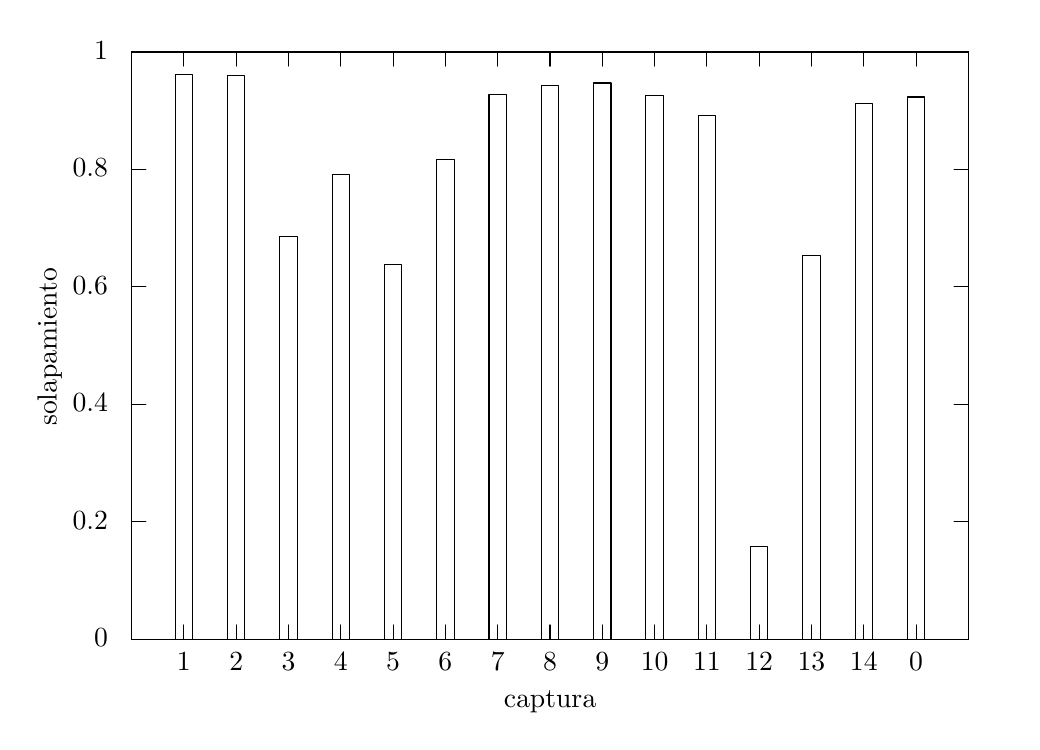
\begin{tikzpicture}[gnuplot]
%% generated with GNUPLOT 5.4p0 (Lua 5.4; terminal rev. Jun 2020, script rev. 114)
%% Tue 25 Aug 2020 01:55:34 AM -03
\gpmonochromelines
\path (0.000,0.000) rectangle (12.500,8.750);
\gpcolor{color=gp lt color border}
\gpsetlinetype{gp lt border}
\gpsetdashtype{gp dt solid}
\gpsetlinewidth{1.00}
\draw[gp path] (1.320,0.985)--(1.500,0.985);
\draw[gp path] (11.947,0.985)--(11.767,0.985);
\node[gp node right] at (1.136,0.985) {$0$};
\draw[gp path] (1.320,2.476)--(1.500,2.476);
\draw[gp path] (11.947,2.476)--(11.767,2.476);
\node[gp node right] at (1.136,2.476) {$0.2$};
\draw[gp path] (1.320,3.967)--(1.500,3.967);
\draw[gp path] (11.947,3.967)--(11.767,3.967);
\node[gp node right] at (1.136,3.967) {$0.4$};
\draw[gp path] (1.320,5.459)--(1.500,5.459);
\draw[gp path] (11.947,5.459)--(11.767,5.459);
\node[gp node right] at (1.136,5.459) {$0.6$};
\draw[gp path] (1.320,6.950)--(1.500,6.950);
\draw[gp path] (11.947,6.950)--(11.767,6.950);
\node[gp node right] at (1.136,6.950) {$0.8$};
\draw[gp path] (1.320,8.441)--(1.500,8.441);
\draw[gp path] (11.947,8.441)--(11.767,8.441);
\node[gp node right] at (1.136,8.441) {$1$};
\draw[gp path] (1.984,0.985)--(1.984,1.165);
\draw[gp path] (1.984,8.441)--(1.984,8.261);
\node[gp node center] at (1.984,0.677) {1};
\draw[gp path] (2.648,0.985)--(2.648,1.165);
\draw[gp path] (2.648,8.441)--(2.648,8.261);
\node[gp node center] at (2.648,0.677) {2};
\draw[gp path] (3.313,0.985)--(3.313,1.165);
\draw[gp path] (3.313,8.441)--(3.313,8.261);
\node[gp node center] at (3.313,0.677) {3};
\draw[gp path] (3.977,0.985)--(3.977,1.165);
\draw[gp path] (3.977,8.441)--(3.977,8.261);
\node[gp node center] at (3.977,0.677) {4};
\draw[gp path] (4.641,0.985)--(4.641,1.165);
\draw[gp path] (4.641,8.441)--(4.641,8.261);
\node[gp node center] at (4.641,0.677) {5};
\draw[gp path] (5.305,0.985)--(5.305,1.165);
\draw[gp path] (5.305,8.441)--(5.305,8.261);
\node[gp node center] at (5.305,0.677) {6};
\draw[gp path] (5.969,0.985)--(5.969,1.165);
\draw[gp path] (5.969,8.441)--(5.969,8.261);
\node[gp node center] at (5.969,0.677) {7};
\draw[gp path] (6.634,0.985)--(6.634,1.165);
\draw[gp path] (6.634,8.441)--(6.634,8.261);
\node[gp node center] at (6.634,0.677) {8};
\draw[gp path] (7.298,0.985)--(7.298,1.165);
\draw[gp path] (7.298,8.441)--(7.298,8.261);
\node[gp node center] at (7.298,0.677) {9};
\draw[gp path] (7.962,0.985)--(7.962,1.165);
\draw[gp path] (7.962,8.441)--(7.962,8.261);
\node[gp node center] at (7.962,0.677) {10};
\draw[gp path] (8.626,0.985)--(8.626,1.165);
\draw[gp path] (8.626,8.441)--(8.626,8.261);
\node[gp node center] at (8.626,0.677) {11};
\draw[gp path] (9.290,0.985)--(9.290,1.165);
\draw[gp path] (9.290,8.441)--(9.290,8.261);
\node[gp node center] at (9.290,0.677) {12};
\draw[gp path] (9.954,0.985)--(9.954,1.165);
\draw[gp path] (9.954,8.441)--(9.954,8.261);
\node[gp node center] at (9.954,0.677) {13};
\draw[gp path] (10.619,0.985)--(10.619,1.165);
\draw[gp path] (10.619,8.441)--(10.619,8.261);
\node[gp node center] at (10.619,0.677) {14};
\draw[gp path] (11.283,0.985)--(11.283,1.165);
\draw[gp path] (11.283,8.441)--(11.283,8.261);
\node[gp node center] at (11.283,0.677) {0};
\draw[gp path] (1.320,8.441)--(1.320,0.985)--(11.947,0.985)--(11.947,8.441)--cycle;
\node[gp node center,rotate=-270] at (0.292,4.713) {solapamiento};
\node[gp node center] at (6.633,0.215) {captura};
\draw[gp path] (1.873,0.985)--(1.873,8.158)--(2.095,8.158)--(2.095,0.985)--cycle;
\draw[gp path] (2.538,0.985)--(2.538,8.144)--(2.759,8.144)--(2.759,0.985)--cycle;
\draw[gp path] (3.202,0.985)--(3.202,6.102)--(3.423,6.102)--(3.423,0.985)--cycle;
\draw[gp path] (3.866,0.985)--(3.866,6.882)--(4.087,6.882)--(4.087,0.985)--cycle;
\draw[gp path] (4.530,0.985)--(4.530,5.745)--(4.752,5.745)--(4.752,0.985)--cycle;
\draw[gp path] (5.194,0.985)--(5.194,7.078)--(5.416,7.078)--(5.416,0.985)--cycle;
\draw[gp path] (5.859,0.985)--(5.859,7.902)--(6.080,7.902)--(6.080,0.985)--cycle;
\draw[gp path] (6.523,0.985)--(6.523,8.015)--(6.744,8.015)--(6.744,0.985)--cycle;
\draw[gp path] (7.187,0.985)--(7.187,8.047)--(7.408,8.047)--(7.408,0.985)--cycle;
\draw[gp path] (7.851,0.985)--(7.851,7.892)--(8.073,7.892)--(8.073,0.985)--cycle;
\draw[gp path] (8.515,0.985)--(8.515,7.634)--(8.737,7.634)--(8.737,0.985)--cycle;
\draw[gp path] (9.180,0.985)--(9.180,2.163)--(9.401,2.163)--(9.401,0.985)--cycle;
\draw[gp path] (9.844,0.985)--(9.844,5.858)--(10.065,5.858)--(10.065,0.985)--cycle;
\draw[gp path] (10.508,0.985)--(10.508,7.788)--(10.729,7.788)--(10.729,0.985)--cycle;
\draw[gp path] (11.172,0.985)--(11.172,7.869)--(11.394,7.869)--(11.394,0.985)--cycle;
\draw[gp path] (1.320,8.441)--(1.320,0.985)--(11.947,0.985)--(11.947,8.441)--cycle;
%% coordinates of the plot area
\gpdefrectangularnode{gp plot 1}{\pgfpoint{1.320cm}{0.985cm}}{\pgfpoint{11.947cm}{8.441cm}}
\end{tikzpicture}
%% gnuplot variables
}
				\resizebox{\linewidth}{!}{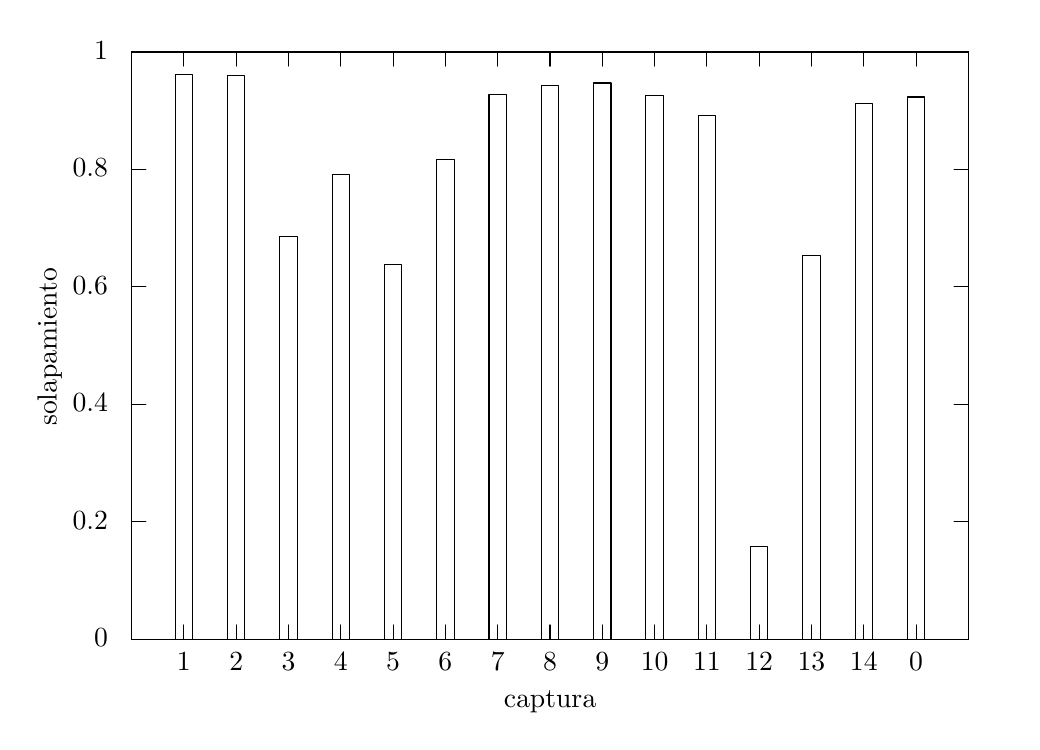
\begin{tikzpicture}[gnuplot]
%% generated with GNUPLOT 5.4p0 (Lua 5.4; terminal rev. Jun 2020, script rev. 114)
%% Tue 25 Aug 2020 01:55:34 AM -03
\gpmonochromelines
\path (0.000,0.000) rectangle (12.500,8.750);
\gpcolor{color=gp lt color border}
\gpsetlinetype{gp lt border}
\gpsetdashtype{gp dt solid}
\gpsetlinewidth{1.00}
\draw[gp path] (1.320,0.985)--(1.500,0.985);
\draw[gp path] (11.947,0.985)--(11.767,0.985);
\node[gp node right] at (1.136,0.985) {$0$};
\draw[gp path] (1.320,2.476)--(1.500,2.476);
\draw[gp path] (11.947,2.476)--(11.767,2.476);
\node[gp node right] at (1.136,2.476) {$0.2$};
\draw[gp path] (1.320,3.967)--(1.500,3.967);
\draw[gp path] (11.947,3.967)--(11.767,3.967);
\node[gp node right] at (1.136,3.967) {$0.4$};
\draw[gp path] (1.320,5.459)--(1.500,5.459);
\draw[gp path] (11.947,5.459)--(11.767,5.459);
\node[gp node right] at (1.136,5.459) {$0.6$};
\draw[gp path] (1.320,6.950)--(1.500,6.950);
\draw[gp path] (11.947,6.950)--(11.767,6.950);
\node[gp node right] at (1.136,6.950) {$0.8$};
\draw[gp path] (1.320,8.441)--(1.500,8.441);
\draw[gp path] (11.947,8.441)--(11.767,8.441);
\node[gp node right] at (1.136,8.441) {$1$};
\draw[gp path] (1.984,0.985)--(1.984,1.165);
\draw[gp path] (1.984,8.441)--(1.984,8.261);
\node[gp node center] at (1.984,0.677) {1};
\draw[gp path] (2.648,0.985)--(2.648,1.165);
\draw[gp path] (2.648,8.441)--(2.648,8.261);
\node[gp node center] at (2.648,0.677) {2};
\draw[gp path] (3.313,0.985)--(3.313,1.165);
\draw[gp path] (3.313,8.441)--(3.313,8.261);
\node[gp node center] at (3.313,0.677) {3};
\draw[gp path] (3.977,0.985)--(3.977,1.165);
\draw[gp path] (3.977,8.441)--(3.977,8.261);
\node[gp node center] at (3.977,0.677) {4};
\draw[gp path] (4.641,0.985)--(4.641,1.165);
\draw[gp path] (4.641,8.441)--(4.641,8.261);
\node[gp node center] at (4.641,0.677) {5};
\draw[gp path] (5.305,0.985)--(5.305,1.165);
\draw[gp path] (5.305,8.441)--(5.305,8.261);
\node[gp node center] at (5.305,0.677) {6};
\draw[gp path] (5.969,0.985)--(5.969,1.165);
\draw[gp path] (5.969,8.441)--(5.969,8.261);
\node[gp node center] at (5.969,0.677) {7};
\draw[gp path] (6.634,0.985)--(6.634,1.165);
\draw[gp path] (6.634,8.441)--(6.634,8.261);
\node[gp node center] at (6.634,0.677) {8};
\draw[gp path] (7.298,0.985)--(7.298,1.165);
\draw[gp path] (7.298,8.441)--(7.298,8.261);
\node[gp node center] at (7.298,0.677) {9};
\draw[gp path] (7.962,0.985)--(7.962,1.165);
\draw[gp path] (7.962,8.441)--(7.962,8.261);
\node[gp node center] at (7.962,0.677) {10};
\draw[gp path] (8.626,0.985)--(8.626,1.165);
\draw[gp path] (8.626,8.441)--(8.626,8.261);
\node[gp node center] at (8.626,0.677) {11};
\draw[gp path] (9.290,0.985)--(9.290,1.165);
\draw[gp path] (9.290,8.441)--(9.290,8.261);
\node[gp node center] at (9.290,0.677) {12};
\draw[gp path] (9.954,0.985)--(9.954,1.165);
\draw[gp path] (9.954,8.441)--(9.954,8.261);
\node[gp node center] at (9.954,0.677) {13};
\draw[gp path] (10.619,0.985)--(10.619,1.165);
\draw[gp path] (10.619,8.441)--(10.619,8.261);
\node[gp node center] at (10.619,0.677) {14};
\draw[gp path] (11.283,0.985)--(11.283,1.165);
\draw[gp path] (11.283,8.441)--(11.283,8.261);
\node[gp node center] at (11.283,0.677) {0};
\draw[gp path] (1.320,8.441)--(1.320,0.985)--(11.947,0.985)--(11.947,8.441)--cycle;
\node[gp node center,rotate=-270] at (0.292,4.713) {solapamiento};
\node[gp node center] at (6.633,0.215) {captura};
\draw[gp path] (1.873,0.985)--(1.873,8.158)--(2.095,8.158)--(2.095,0.985)--cycle;
\draw[gp path] (2.538,0.985)--(2.538,8.144)--(2.759,8.144)--(2.759,0.985)--cycle;
\draw[gp path] (3.202,0.985)--(3.202,6.102)--(3.423,6.102)--(3.423,0.985)--cycle;
\draw[gp path] (3.866,0.985)--(3.866,6.882)--(4.087,6.882)--(4.087,0.985)--cycle;
\draw[gp path] (4.530,0.985)--(4.530,5.745)--(4.752,5.745)--(4.752,0.985)--cycle;
\draw[gp path] (5.194,0.985)--(5.194,7.078)--(5.416,7.078)--(5.416,0.985)--cycle;
\draw[gp path] (5.859,0.985)--(5.859,7.902)--(6.080,7.902)--(6.080,0.985)--cycle;
\draw[gp path] (6.523,0.985)--(6.523,8.015)--(6.744,8.015)--(6.744,0.985)--cycle;
\draw[gp path] (7.187,0.985)--(7.187,8.047)--(7.408,8.047)--(7.408,0.985)--cycle;
\draw[gp path] (7.851,0.985)--(7.851,7.892)--(8.073,7.892)--(8.073,0.985)--cycle;
\draw[gp path] (8.515,0.985)--(8.515,7.634)--(8.737,7.634)--(8.737,0.985)--cycle;
\draw[gp path] (9.180,0.985)--(9.180,2.163)--(9.401,2.163)--(9.401,0.985)--cycle;
\draw[gp path] (9.844,0.985)--(9.844,5.858)--(10.065,5.858)--(10.065,0.985)--cycle;
\draw[gp path] (10.508,0.985)--(10.508,7.788)--(10.729,7.788)--(10.729,0.985)--cycle;
\draw[gp path] (11.172,0.985)--(11.172,7.869)--(11.394,7.869)--(11.394,0.985)--cycle;
\draw[gp path] (1.320,8.441)--(1.320,0.985)--(11.947,0.985)--(11.947,8.441)--cycle;
%% coordinates of the plot area
\gpdefrectangularnode{gp plot 1}{\pgfpoint{1.320cm}{0.985cm}}{\pgfpoint{11.947cm}{8.441cm}}
\end{tikzpicture}
%% gnuplot variables
}
			\caption{\label{fig:fitness}Métrica de alineación para el modelo \texttt{dragon stand}. El bajo
			porcentaje de solapamiento en la captura 12 se corresponde
			con un error de registración.}
		\end{figure}



		Como medida de error de la fusión se utilizó la distancia entre los puntos de la nube reconstruida
		respecto al punto más cercano en el \emph{ground truth} (cuadro~\ref{tab:fus_error}).
		La reconstrucción del modelo \texttt{armadillo} se encontraba a otra
		escala, por lo que no fue utilizada.
		Nuevamente se destaca el error de \texttt{dragon stand} producto de una mala alineación.

		\begin{table}
	\center
	\begin{tabular}{l*{3}{c}}
		\toprule                                                                  
		Modelo                  &    Error promedio  & Desvío \\ 
		\midrule                                    
		bunny                   &      1.28464       & 0.74131\\
		\midrule                                    
		dragon side             &      1.19651       & 0.69846\\
		dragon stand            &      2.83930       & 2.41398\\
		dragon up               &      1.14363       & 0.88966\\
		\midrule                                    
		drill (contra vrip)     &      1.48515       & 0.96336\\
		drill (contra zip)      &      1.74326       & 1.39883\\
		\midrule                                    
		happy back              &      1.65632       & 1.27056\\
		happy side              &      1.35371       & 1.01163\\
		happy stand             &      1.79513       & 1.25758\\
		\bottomrule                                                               
	\end{tabular}
	\caption{\label{tab:fus_error}Errores en la fusión.}
\end{table}



		%gráficos drill y front/back
		%En el caso de \texttt{drill}, 

		%solo front/back
		Se observa, además, una inflación/deflación de los objetos
		reconstruidos debida a la propagación del error de alineación.  Así, la
		primera captura coincide casi exactamente, pero el error se incrementa
		a medida que nos alejamos de ella (figura~\ref{fig:fus_happy}).

		\begin{figure}
			\Imagen{happy_diff}
			\caption{\label{fig:fus_happy}Diferencia contra el \emph{ground truth} del modelo \texttt{happy}.}
		\end{figure}


		%rellenado de huecos poisson
		Luego de aplicar el método de Poisson para rellenar los huecos, se
		obtuvieron las reconstrucciones que se observan en la
		figura~\ref{fig:poiss_all}.
		Los desperfectos observados en bunny (figura~\ref{fig:bun_ear}) se deben a una mala registración
		de la captura \texttt{bun180}, que se encontraba aproximadamente a
		$90^{\circ}$ respecto a sus vecinos.
		En cuanto a drill (figura~\ref{fig:drill_drops}), se tienen componentes
		inconexas debido a una mala fusión en una zona de alta curvatura.
		En todos los casos, la base de apoyo del objeto presenta una
		deformación hacia abajo (figura~\ref{fig:base}) con un hueco al final.
		Esto podría solucionarse mediante un preproceso rellenando la base con,
		por ejemplo, el método de \emph{advancing front}.

		\begin{figure}
			\Imagen{img/models_b}
			\caption{\label{fig:poiss_all}Resultado de las reconstrucciones luego del rellenado de huecos mediante el método de Poisson.
			Fila superior:
			De izquierda a derecha, y de arriba a abajo, los modelos son: armadillo, bunny, dragon, drill y happy.}
		\end{figure}

		\begin{figure}
			\centering
			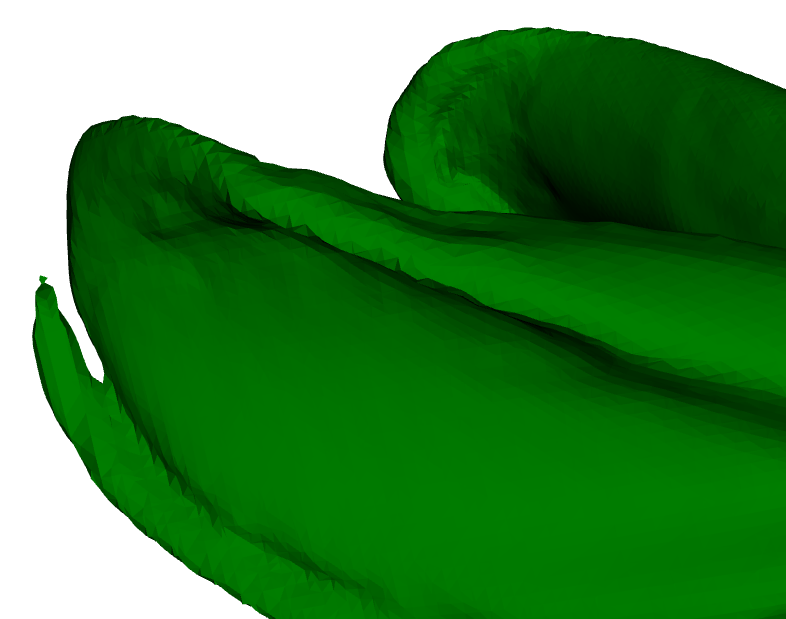
\includegraphics[max width=.5\linewidth, max height=.25\textheight, keepaspectratio]
				{img/bunny_ear}
			%\Imagen{img/bunny_ear}
			\caption{\label{fig:bun_ear}Acercamiento a la oreja derecha de bunny.}
		\end{figure}

		\begin{figure}
			%\Imagen{img/drill_drops}
			\centering
			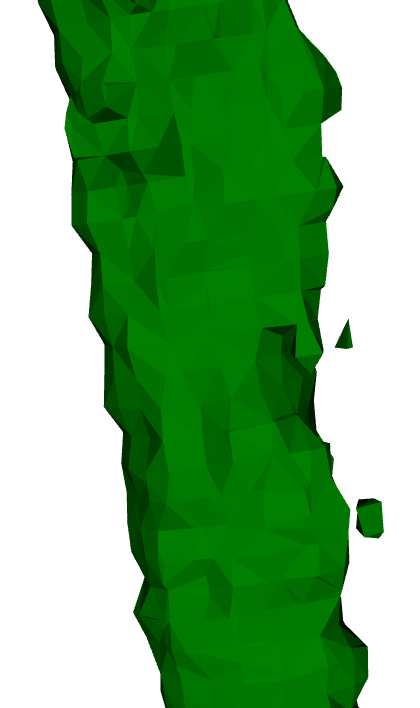
\includegraphics[max width=.5\linewidth, max height=.25\textheight, keepaspectratio]
				{img/drill_drops}
			\caption{\label{fig:drill_drops}Acercamiento a la mecha de drill. Se observan componentes inconexas con la malla principal.}
		\end{figure}

		\begin{figure}
			\centering
			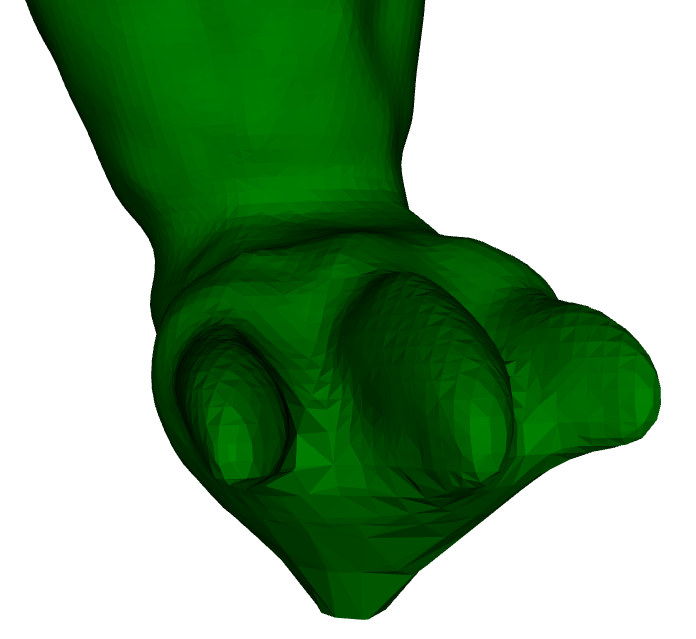
\includegraphics[max width=.5\linewidth, max height=.25\textheight, keepaspectratio]
				{img/arma_foot}
			%\Imagen{img/arma_foot}
			\caption{\label{fig:base}Acercamiento a la base de apoyo de armadillo. Se observa un estiramiento hacia abajo.}
		\end{figure}



	\section{Conclusiones}
		Como resultado de esta etapa se obtuvo una biblioteca de software que
		permite reconstruir un objeto tridimensional a partir de nubes
		de puntos de vistas parciales sujetas a ciertas restricciones.
		Debido al uso del método de Poisson en el rellenado, esta
		reconstrucción no presentará huecos, a excepción de la base de apoyo.

		Durante la registración, se obtuvieron resultados aceptables en casi todas las pruebas, 
		siendo uno de los fallos debido a un ángulo excesivo entre las tomas.
		Estos fallos pueden detectarse al utilizar la métrica de solapamiento y entonces proceder
		a ajustar los parámetros del algoritmo de alineación.

		A futuro se pretende desarrollar algoritmos que nos permitan relajar la
		restricción del eje de giro.
		De esta forma, se podrán combinar reconstrucciones del mismo objeto
		sobre la base de giro, con lo que se logrará recuperar la información
		perdida debido a oclusiones.




	\chapter{Pruebas y resultados}
	A continuación se detallan las pruebas realizadas y los resultados obtenidos
	por cada módulo desarrollado utilizando como base los modelos
	\texttt{armadillo}, \texttt{bunny}, \texttt{dragon}, \texttt{drill} y \texttt{happy}
	del repositorio de Stanford\cite{StanfordScanRep}.

	\section{Módulo de registración}
	Para la registración se utilizó el método basado en la búsqueda de clúster,
	seguido de un refinamiento mediante ICP y una corrección de bucle.
	Se plantearon dos métodos para evaluar la calidad de cada registración:
	\begin{itemize}
		\item Mediante la comparación entre la transformación calculada y aquella provista por la base de datos (\emph{ground truth}).
		\item Mediante una métrica de \emph{fitness} que se obtiene a partir de la nube transformada y las nubes de entrada.
	\end{itemize}

	Para comparar las alineaciones contra el \emph{ground truth}, se
	observa el efecto de las mismas sobre un punto orientado simulando la
	cámara (figura~\ref{fig:err_reg}). El punto \emph{eye} ($C$) se ubica inicialmente en las coordenadas
	$\{0, -0.1, 0.7\}$ (valores obtenidos de la base de datos), y se
	orienta el vector \emph{target} hacia $-z$ y el \emph{up} hacia $y$.
	El error de posicionamiento es la razón entre la distancia al punto
	de inicio y la distancia al punto obtenido por el \emph{ground truth}.
	\[\text{Error} = \frac{|C'-C_{gt}|}{|C_{gt} - C|}\]
	Los errores de \emph{target} y \emph{up} se corresponden al ángulo formado contra los
	vectores respectivos obtenidos por el \emph{ground truth}.

	\begin{figure}
		\centering
		\input{diagram/error_registration.pdf_tex}
		\caption{\label{fig:err_reg}Comparación entre las transformaciones de alineación.
		Se observa el efecto producido en un punto orientado $C$ que simula la posición de la cámara.}
	\end{figure}

	En el cuadro~\ref{tab:reg_error} se presentan los errores de registración promedio para cada orientación de los modelos.
	En la mayoría de los casos, los errores no superan $1^{\circ}$ en orientación ni $1\%$ en posicionamiento,
	observándose dos excepciones: \texttt{bunny} y \texttt{dragon stand}.
	El aumento en el error del modelo \texttt{bunny} se debe a que la captura \texttt{bun180} presenta una distancia cercana a $90^\circ$,
	superando las restricciones impuestas en este trabajo.
	Sin embargo, en el caso de \texttt{dragon stand} el error refleja una mala
	alineación en la captura~12, debida a una mala selección de los parámetros.
	Mediante un posterior ajuste de los parámetros, en particular, del tamaño de la vecindad para el cálculo de los descriptores, se obtuvo una alineación correcta.

	\begin{table}
	\centering
	\begin{tabular}{l*{3}{c}}
		\toprule                                                                  
		Modelo                   &    Eye          &    Target (grados)        &    Up (grados)\\
		\midrule
		armadillo back          &     0.0062159   &   0.221725     &    ---\\        
		armadillo head          &     0.0036356  &    0.102321     &    0.211231\\   
		armadillo head offset   &     0.0029806  &    0.086309     &    0.229574\\   
		armadillo stand         &     0.0022145  &    0.049612     &    0.105862\\   
		armadillo stand flip    &     0.0045019  &    0.125330     &    0.146033\\   
		\midrule
		bunny                   &     0.0104809   &   0.598354     &    0.817185\\   
		\midrule
		dragon side             &     0.0070872  &    0.178650     &    0.212932\\   
		dragon stand            &     0.0536199   &   1.379760     &    0.207754\\   
		dragon up               &     0.0058265  &    0.139297     &    ---\\        
		\midrule
		drill                   &     0.0082317  &    0.238639     &    0.100126\\   
		\midrule
		happy back              &     0.0088540  &    0.189885     &    0.207247\\   
		happy side              &     0.0072675   &   0.175860     &    ---\\        
		happy stand             &     0.0050124  &    0.101383     &    0.097800\\  
		\bottomrule                                                               
	\end{tabular}
	\caption[Errores de registración]{\label{tab:reg_error}Errores de registración.
	\TODO{¿por qué hay vacíos?}}
\end{table}


	Para evaluar la alineación entre un par de capturas prescindiendo del \emph{ground truth}, y situándonos en un escenario más realista,
	se diseñó una medida de \emph{fitness}.
	Esta medida se define como el porcentaje del área solapada entre las nubes una vez alineadas,
	donde un bajo solapamiento nos indicaría un posible error de alineación, como
	se observa en la figura~\ref{fig:fitness}.

	\begin{figure}
		\centering
			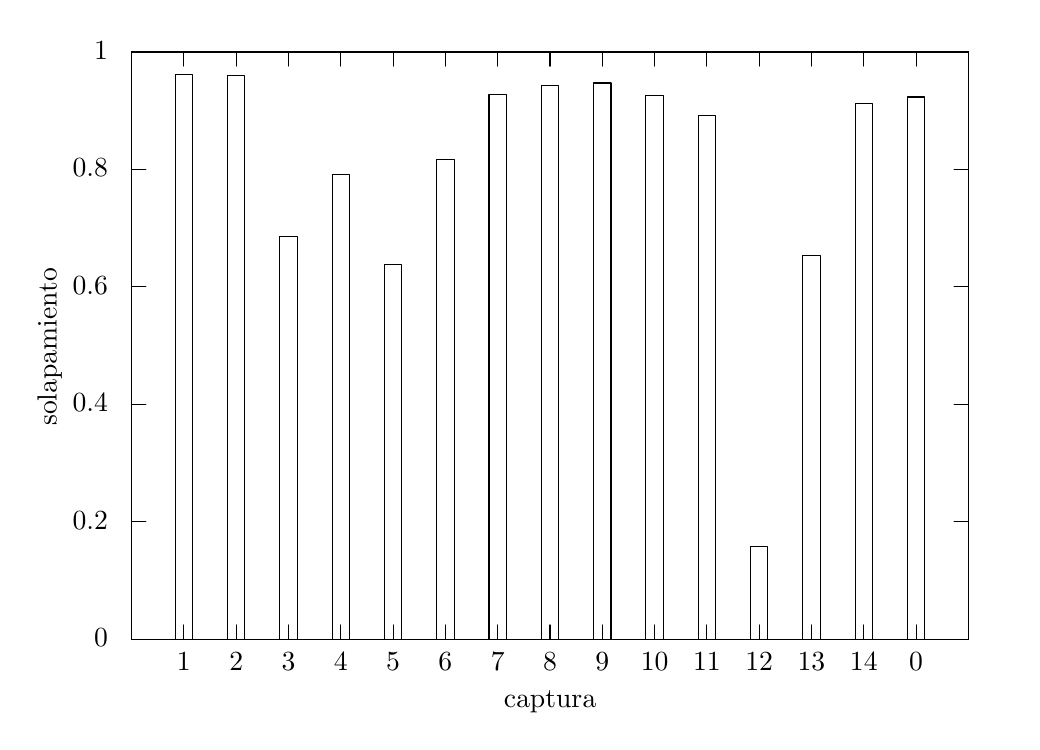
\begin{tikzpicture}[gnuplot]
%% generated with GNUPLOT 5.4p0 (Lua 5.4; terminal rev. Jun 2020, script rev. 114)
%% Tue 25 Aug 2020 01:55:34 AM -03
\gpmonochromelines
\path (0.000,0.000) rectangle (12.500,8.750);
\gpcolor{color=gp lt color border}
\gpsetlinetype{gp lt border}
\gpsetdashtype{gp dt solid}
\gpsetlinewidth{1.00}
\draw[gp path] (1.320,0.985)--(1.500,0.985);
\draw[gp path] (11.947,0.985)--(11.767,0.985);
\node[gp node right] at (1.136,0.985) {$0$};
\draw[gp path] (1.320,2.476)--(1.500,2.476);
\draw[gp path] (11.947,2.476)--(11.767,2.476);
\node[gp node right] at (1.136,2.476) {$0.2$};
\draw[gp path] (1.320,3.967)--(1.500,3.967);
\draw[gp path] (11.947,3.967)--(11.767,3.967);
\node[gp node right] at (1.136,3.967) {$0.4$};
\draw[gp path] (1.320,5.459)--(1.500,5.459);
\draw[gp path] (11.947,5.459)--(11.767,5.459);
\node[gp node right] at (1.136,5.459) {$0.6$};
\draw[gp path] (1.320,6.950)--(1.500,6.950);
\draw[gp path] (11.947,6.950)--(11.767,6.950);
\node[gp node right] at (1.136,6.950) {$0.8$};
\draw[gp path] (1.320,8.441)--(1.500,8.441);
\draw[gp path] (11.947,8.441)--(11.767,8.441);
\node[gp node right] at (1.136,8.441) {$1$};
\draw[gp path] (1.984,0.985)--(1.984,1.165);
\draw[gp path] (1.984,8.441)--(1.984,8.261);
\node[gp node center] at (1.984,0.677) {1};
\draw[gp path] (2.648,0.985)--(2.648,1.165);
\draw[gp path] (2.648,8.441)--(2.648,8.261);
\node[gp node center] at (2.648,0.677) {2};
\draw[gp path] (3.313,0.985)--(3.313,1.165);
\draw[gp path] (3.313,8.441)--(3.313,8.261);
\node[gp node center] at (3.313,0.677) {3};
\draw[gp path] (3.977,0.985)--(3.977,1.165);
\draw[gp path] (3.977,8.441)--(3.977,8.261);
\node[gp node center] at (3.977,0.677) {4};
\draw[gp path] (4.641,0.985)--(4.641,1.165);
\draw[gp path] (4.641,8.441)--(4.641,8.261);
\node[gp node center] at (4.641,0.677) {5};
\draw[gp path] (5.305,0.985)--(5.305,1.165);
\draw[gp path] (5.305,8.441)--(5.305,8.261);
\node[gp node center] at (5.305,0.677) {6};
\draw[gp path] (5.969,0.985)--(5.969,1.165);
\draw[gp path] (5.969,8.441)--(5.969,8.261);
\node[gp node center] at (5.969,0.677) {7};
\draw[gp path] (6.634,0.985)--(6.634,1.165);
\draw[gp path] (6.634,8.441)--(6.634,8.261);
\node[gp node center] at (6.634,0.677) {8};
\draw[gp path] (7.298,0.985)--(7.298,1.165);
\draw[gp path] (7.298,8.441)--(7.298,8.261);
\node[gp node center] at (7.298,0.677) {9};
\draw[gp path] (7.962,0.985)--(7.962,1.165);
\draw[gp path] (7.962,8.441)--(7.962,8.261);
\node[gp node center] at (7.962,0.677) {10};
\draw[gp path] (8.626,0.985)--(8.626,1.165);
\draw[gp path] (8.626,8.441)--(8.626,8.261);
\node[gp node center] at (8.626,0.677) {11};
\draw[gp path] (9.290,0.985)--(9.290,1.165);
\draw[gp path] (9.290,8.441)--(9.290,8.261);
\node[gp node center] at (9.290,0.677) {12};
\draw[gp path] (9.954,0.985)--(9.954,1.165);
\draw[gp path] (9.954,8.441)--(9.954,8.261);
\node[gp node center] at (9.954,0.677) {13};
\draw[gp path] (10.619,0.985)--(10.619,1.165);
\draw[gp path] (10.619,8.441)--(10.619,8.261);
\node[gp node center] at (10.619,0.677) {14};
\draw[gp path] (11.283,0.985)--(11.283,1.165);
\draw[gp path] (11.283,8.441)--(11.283,8.261);
\node[gp node center] at (11.283,0.677) {0};
\draw[gp path] (1.320,8.441)--(1.320,0.985)--(11.947,0.985)--(11.947,8.441)--cycle;
\node[gp node center,rotate=-270] at (0.292,4.713) {solapamiento};
\node[gp node center] at (6.633,0.215) {captura};
\draw[gp path] (1.873,0.985)--(1.873,8.158)--(2.095,8.158)--(2.095,0.985)--cycle;
\draw[gp path] (2.538,0.985)--(2.538,8.144)--(2.759,8.144)--(2.759,0.985)--cycle;
\draw[gp path] (3.202,0.985)--(3.202,6.102)--(3.423,6.102)--(3.423,0.985)--cycle;
\draw[gp path] (3.866,0.985)--(3.866,6.882)--(4.087,6.882)--(4.087,0.985)--cycle;
\draw[gp path] (4.530,0.985)--(4.530,5.745)--(4.752,5.745)--(4.752,0.985)--cycle;
\draw[gp path] (5.194,0.985)--(5.194,7.078)--(5.416,7.078)--(5.416,0.985)--cycle;
\draw[gp path] (5.859,0.985)--(5.859,7.902)--(6.080,7.902)--(6.080,0.985)--cycle;
\draw[gp path] (6.523,0.985)--(6.523,8.015)--(6.744,8.015)--(6.744,0.985)--cycle;
\draw[gp path] (7.187,0.985)--(7.187,8.047)--(7.408,8.047)--(7.408,0.985)--cycle;
\draw[gp path] (7.851,0.985)--(7.851,7.892)--(8.073,7.892)--(8.073,0.985)--cycle;
\draw[gp path] (8.515,0.985)--(8.515,7.634)--(8.737,7.634)--(8.737,0.985)--cycle;
\draw[gp path] (9.180,0.985)--(9.180,2.163)--(9.401,2.163)--(9.401,0.985)--cycle;
\draw[gp path] (9.844,0.985)--(9.844,5.858)--(10.065,5.858)--(10.065,0.985)--cycle;
\draw[gp path] (10.508,0.985)--(10.508,7.788)--(10.729,7.788)--(10.729,0.985)--cycle;
\draw[gp path] (11.172,0.985)--(11.172,7.869)--(11.394,7.869)--(11.394,0.985)--cycle;
\draw[gp path] (1.320,8.441)--(1.320,0.985)--(11.947,0.985)--(11.947,8.441)--cycle;
%% coordinates of the plot area
\gpdefrectangularnode{gp plot 1}{\pgfpoint{1.320cm}{0.985cm}}{\pgfpoint{11.947cm}{8.441cm}}
\end{tikzpicture}
%% gnuplot variables

		\caption[Métrica de alineación para el modelo \texttt{dragon stand}]{\label{fig:fitness}Métrica de alineación para el modelo \texttt{dragon stand}. El bajo
		porcentaje de solapamiento en la captura 12 se corresponde
		con un error de registración.}
	\end{figure}


	\section{Módulo de fusión}
	%En la fusión se utilizó una distancia de proximidad de $1.5$ veces la resolución de las nubes,
	%y un mínimo de confianza de $0.2$.

	Como medida de error de la fusión se utilizó la distancia entre los puntos de la nube reconstruida
	respecto al punto más cercano en el \emph{ground truth} (cuadro~\ref{tab:fus_error}).
	Esta medición no se realizó para el modelo \texttt{armadillo} debido a que su reconstrucción
	se encontraba a una escala distinta a la de las capturas.
	Nuevamente se destaca el error de \texttt{dragon stand} producto de una mala alineación.

	\begin{table}
	\center
	\begin{tabular}{l*{3}{c}}
		\toprule                                                                  
		Modelo                  &    Error promedio  & Desvío \\ 
		\midrule                                    
		bunny                   &      1.28464       & 0.74131\\
		\midrule                                    
		dragon side             &      1.19651       & 0.69846\\
		dragon stand            &      2.83930       & 2.41398\\
		dragon up               &      1.14363       & 0.88966\\
		\midrule                                    
		drill (contra vrip)     &      1.48515       & 0.96336\\
		drill (contra zip)      &      1.74326       & 1.39883\\
		\midrule                                    
		happy back              &      1.65632       & 1.27056\\
		happy side              &      1.35371       & 1.01163\\
		happy stand             &      1.79513       & 1.25758\\
		\bottomrule                                                               
	\end{tabular}
	\caption{\label{tab:fus_error}Errores en la fusión.}
\end{table}



	En todos los modelos, se observa, además, una inflación/deflación de los objetos
	reconstruidos debida a la propagación del error de alineación.  Así, la
	primera captura coincide casi exactamente, pero el error se incrementa
	a medida que nos alejamos de ella (figura~\ref{fig:fus_happy}).

	\begin{figure}
		\Imagen{img/happy_diff}
		\caption[Medida de error en la fusión]{\label{fig:fus_happy}Diferencia contra el \emph{ground truth} del modelo \texttt{happy}.}
	\end{figure}

	\section{Módulo de rellenado de huecos}
		\subsection{Método de advancing front}
		Al utilizar el método de advancing front sobre la superficie reconstruida de \texttt{bunny},
		se logró el rellenado de agujeros pequeños, obteniéndose una malla regular (figura~\ref{fig:fill_good}).
		Sin embargo, debido a la localidad con la que se generan los nuevos
		puntos, el frente puede diverger o pretender unirse a puntos que no
		forman parte del contorno del hueco, resultando una malla mal formada,
		con aristas que corresponden a más de dos caras (figura~\ref{fig:fill_bad}).
		Por estas razones, el método no resulta adecuado para el rellenado automático.


		\begin{figure}
			\Imagen{img/fill_good}
			\caption[Relleno de un hueco pequeño mediante \emph{advancing front}]
			{\label{fig:fill_good}Relleno de un hueco pequeño mediante \emph{advancing front}.}
		\end{figure}

		\begin{figure}
			\Imagen{img/fill_bad}
			\caption[Fallo en el algoritmo de \emph{advancing front}]
			{\label{fig:fill_bad}Fallo en el algoritmo de \emph{advancing front}.
			Se intentó completar un triángulo con un punto que no pertenecía al borde.}
		\end{figure}

		\subsection{Reconstrucción de Poisson}
		Como se mencionó anteriormente, la reconstrucción de Poisson nos garantiza el
		rellenado de todos los huecos (a excepción de la base) mediante una superficie suave.
		Se procedió, entonces, a una valoración visual de los objetos reconstruidos (figura~\ref{fig:poiss_all}):
		\begin{itemize}
			\item En \texttt{bunny} (figura~\ref{fig:bun_ear}) se observan desperfectos debidos a una mala registración de la captura \texttt{bun180},
				que se encontraba aproximadamente a $90^{\circ}$ respecto a sus vecinos.
			\item En \texttt{drill} (figura~\ref{fig:drill_drops}) se tienen componentes inconexas debido a una mala fusión en una zona de alta curvatura.
			\item En \texttt{dragon}(figura~\ref{fig:dragon_belly}) se observa la creación de un puente entre dos regiones.
				Esta es una de las limitaciones conocidas del método, al no poder incorporar la información de línea de vista de las capturas\cite{Kazhdan:2006:PSR:1281957.1281965}.
			\item En todos los casos, la base de apoyo del objeto presenta una deformación hacia abajo (figura~\ref{fig:base}) con un hueco al final.
		\end{itemize}

		\begin{figure}
			\Imagen{img/models_b}
			\caption[Resultado de las reconstrucciones]{\label{fig:poiss_all}Resultado de las reconstrucciones luego del rellenado de huecos mediante el método de Poisson.
			De izquierda a derecha y de arriba a abajo, los modelos son:
			\texttt{armadillo},
			\texttt{bunny},
			\texttt{dragon},
			\texttt{drill}
			y \texttt{happy}.}
		\end{figure}

		\begin{figure}
			\centering
			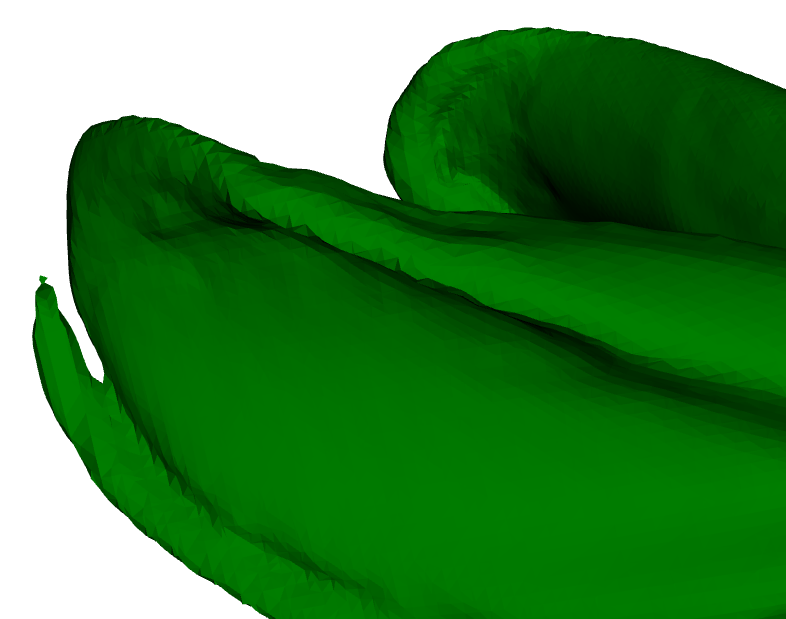
\includegraphics[max width=.5\linewidth, max height=.25\textheight, keepaspectratio]
				{img/bunny_ear}
			%\Imagen{img/bunny_ear}
			\caption[Acercamiento a la oreja derecha de \texttt{bunny}]{\label{fig:bun_ear}Acercamiento a la oreja derecha de \texttt{bunny}.}
		\end{figure}

		\begin{figure}
			%\Imagen{img/drill_drops}
			\centering
			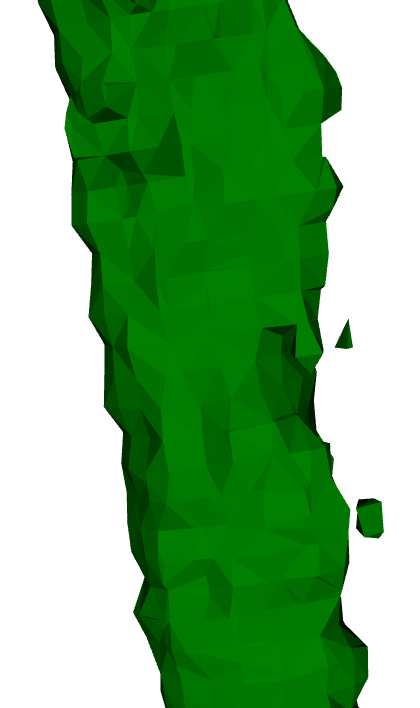
\includegraphics[max width=.5\linewidth, max height=.25\textheight, keepaspectratio]
				{img/drill_drops}
			\caption[Acercamiento a la mecha de \texttt{drill}]{\label{fig:drill_drops}Acercamiento a la mecha de \texttt{drill}.}
		\end{figure}

		\begin{figure}
			%\Imagen{img/drill_drops}
			\centering
			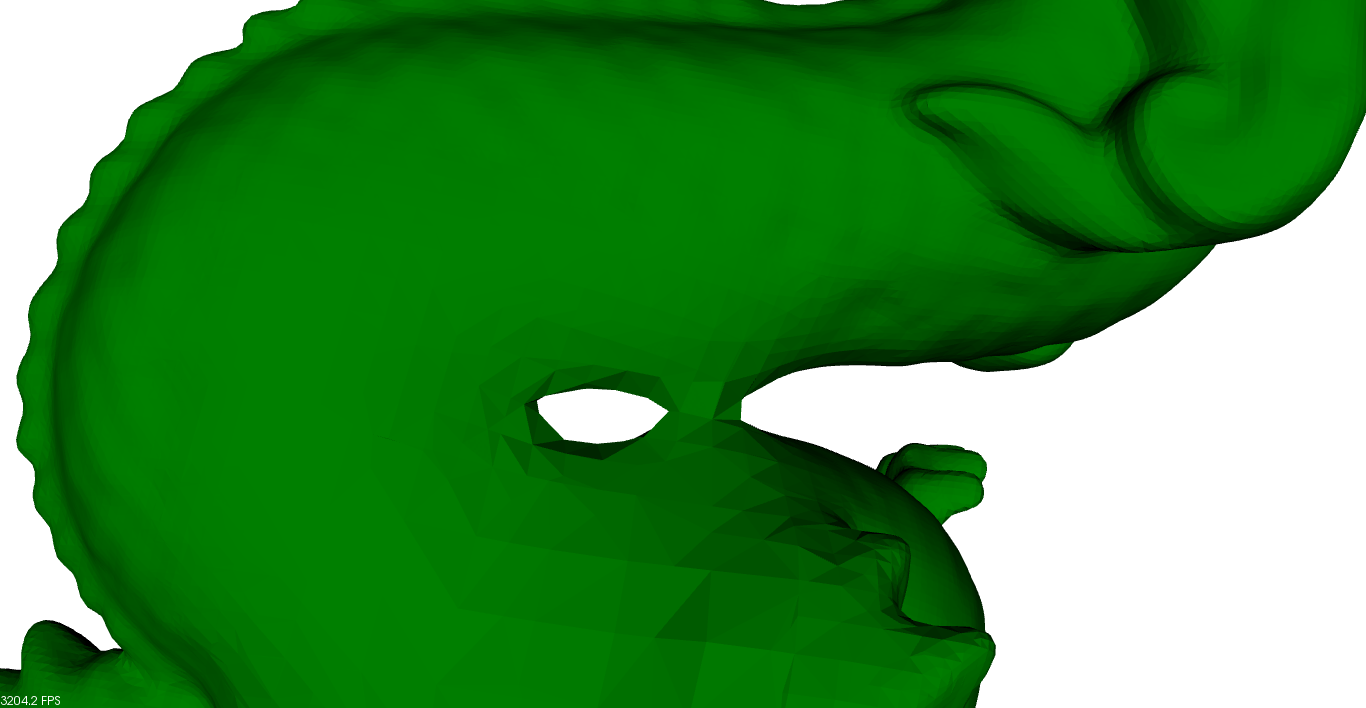
\includegraphics[max width=.5\linewidth, max height=.25\textheight, keepaspectratio]
				{img/dragon_belly}
			\caption[Acercamiento al vientre de \texttt{dragon}]{\label{fig:dragon_belly}Acercamiento al vientre de \texttt{dragon}.}
		\end{figure}

		\begin{figure}
			\centering
			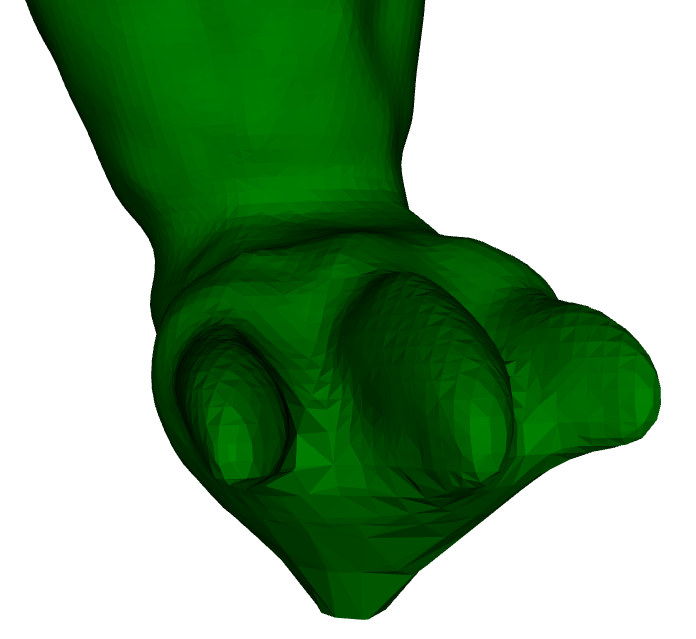
\includegraphics[max width=.5\linewidth, max height=.25\textheight, keepaspectratio]
				{img/arma_foot}
			%\Imagen{img/arma_foot}
			\caption[Acercamiento a la base de apoyo de \texttt{armadillo}]{\label{fig:base}Acercamiento a la base de apoyo de \texttt{armadillo}. Se observa un estiramiento hacia abajo debido al uso de condiciones de borde Neumann.}
		\end{figure}

		%trabajo futuro (advancing front)
		%Para evitar la divergencia es necesario definir una superficie de
		%soporte considerando todo el contorno del hueco, de forma de asegurar
		%que los nuevos puntos no excedan los límites del hueco.

	\section{Tiempo de ejecución}
		Durante el proceso de reconstrucción, se observa que la etapa de reconstrucción
		es responsable de la mayor parte del costo computacional, sobre todo al aumentar
		la cantidad de puntos en las capturas (cuadro~\ref{tab:reconstr_time}).
		En el cuadro~\ref{tab:reg_time} se muestran
		los tiempos de ejecución promedio, discriminados en la alineación
		inicial y el refinamiento posterior.
		El orden $\bigO\left(n^2\right)$ de la alineación inicial se debe a la búsqueda
		entre todos los pares de puntos para establecer las correspondencias (figura~\ref{fig:registration_order}).
		%Si bien los tiempos no son considerables, pueden reducirse al mejorar
		%la selección inicial de puntos y realizar la búsqueda de las
		%correspondencias de forma más eficiente.
		\begin{table}
	\centering
	\begin{tabular}{l*{6}{r}}
		\toprule
		Modelo                 & Puntos   & Capturas  &  Registración & Fusión   & Rellenado & Total\\
		\midrule
		armadillo back         &  25e3    &   11      &   84.4308        & 10.759  &  8.562  & 103.752\\
		armadillo head         &  25e3    &   12      &   114.4926       & 12.501  &  9.892  & 136.886\\
		armadillo head offset  &  25e3    &   11      &   100.7846       & 11.987  &  9.718  & 122.490\\
		armadillo stand        &  25e3    &   12      &   102.3553       & 12.145  &  9.498  & 123.998\\
		armadillo stand flip   &  25e3    &   11      &   101.7061       & 12.958  &  9.280  & 123.944\\
		\midrule
		bunny                  &  35e3    &   6       &    92.2872       & 11.246  &  11.862 & 115.395\\
		\midrule
		dragon side            &  20e3    &   15      &   90.5427        & 14.021  &  8.086  & 112.650\\
		dragon stand           &  30e3    &   15      &   180.8010       & 23.485  &  12.680 & 216.966\\
		dragon up              &  30e3    &   15      &   164.1075       & 18.469  &  9.669  & 192.245\\
		\midrule
		drill                  &   4e3    &   12      &   4.3172         & 1.988   &  4.176  & 10.481 \\
		\midrule
		happy back             &  45e3    &   15      &   343.2705       & 29.618  &  7.528  & 380.417\\
		happy side             &  45e3    &   15      &   452.5830       & 32.588  &  8.361  & 493.532\\
		happy stand            &  75e3    &   15      &   907.2930       & 44.570  &  10.929 & 962.792\\
		\bottomrule
	\end{tabular}
	\caption[Tiempo de reconstrucción]{\label{tab:reconstr_time}Tiempo de reconstrucción por cada modelo (en segundos).}
\end{table}



		\begin{table}
	\centering
	\begin{tabular}{l*{4}{c}}
		\toprule
		Modelo                 &  Puntos  &   Inicial (s)  &   ICP  (s)  &  Total  (s)\\
		\midrule
		armadillo\\
		{\Em}back         &  25e3    &       7.05694    &   0.618592  &    7.67553\\
		{\Em}head         &  25e3    &       8.94947    &   0.591576  &    9.54105\\
		{\Em}head offset  &  25e3    &       8.62241    &   0.539835  &    9.16224\\
		{\Em}stand        &  25e3    &       7.98686    &   0.542746  &    8.52961\\
		{\Em}stand flip   &  25e3    &       8.69949    &   0.546518  &    9.24601\\
		\midrule
		bunny                  &  35e3    &       14.0323    &   1.348890  &    15.3812\\
		\midrule
		dragon\\
		{\Em}side            &  20e3    &       5.52965    &   0.506529  &    6.03618\\
		{\Em}stand           &  30e3    &       11.3732    &   0.680195  &    12.0534\\
		{\Em}up              &  30e3    &       10.3322    &   0.608282  &    10.9405\\
		\midrule
		drill                  &   4e3    &       0.26898    &   0.090796  &    0.35977\\
		\midrule
		happy\\
		{\Em}back             &  45e3    &       21.2702    &   1.614520  &    22.8847\\
		{\Em}side             &  45e3    &       29.1103    &   1.061880  &    30.1722\\
		{\Em}stand            &  75e3    &       59.3281    &   1.158030  &    60.4862\\
		\bottomrule
	\end{tabular}
	\caption[Tiempos de ejecución promedio para la registración]{\label{tab:reg_time}Tiempos de ejecución promedio para la
	registración de a pares en los distintos modelos.}
\end{table}


		\begin{figure}
			\centering
			\begin{tikzpicture}[gnuplot]
%% generated with GNUPLOT 5.4p0 (Lua 5.4; terminal rev. Jun 2020, script rev. 114)
%% Thu 27 Aug 2020 10:08:06 PM -03
\gpmonochromelines
\path (0.000,0.000) rectangle (12.500,8.750);
\gpcolor{color=gp lt color border}
\gpsetlinetype{gp lt border}
\gpsetdashtype{gp dt solid}
\gpsetlinewidth{1.00}
\draw[gp path] (1.504,0.985)--(1.684,0.985);
\draw[gp path] (11.947,0.985)--(11.767,0.985);
\node[gp node right] at (1.320,0.985) {$10^{-2}$};
\draw[gp path] (1.504,1.546)--(1.594,1.546);
\draw[gp path] (11.947,1.546)--(11.857,1.546);
\draw[gp path] (1.504,1.874)--(1.594,1.874);
\draw[gp path] (11.947,1.874)--(11.857,1.874);
\draw[gp path] (1.504,2.107)--(1.594,2.107);
\draw[gp path] (11.947,2.107)--(11.857,2.107);
\draw[gp path] (1.504,2.288)--(1.594,2.288);
\draw[gp path] (11.947,2.288)--(11.857,2.288);
\draw[gp path] (1.504,2.435)--(1.594,2.435);
\draw[gp path] (11.947,2.435)--(11.857,2.435);
\draw[gp path] (1.504,2.560)--(1.594,2.560);
\draw[gp path] (11.947,2.560)--(11.857,2.560);
\draw[gp path] (1.504,2.668)--(1.594,2.668);
\draw[gp path] (11.947,2.668)--(11.857,2.668);
\draw[gp path] (1.504,2.764)--(1.594,2.764);
\draw[gp path] (11.947,2.764)--(11.857,2.764);
\draw[gp path] (1.504,2.849)--(1.684,2.849);
\draw[gp path] (11.947,2.849)--(11.767,2.849);
\node[gp node right] at (1.320,2.849) {$10^{-1}$};
\draw[gp path] (1.504,3.410)--(1.594,3.410);
\draw[gp path] (11.947,3.410)--(11.857,3.410);
\draw[gp path] (1.504,3.738)--(1.594,3.738);
\draw[gp path] (11.947,3.738)--(11.857,3.738);
\draw[gp path] (1.504,3.971)--(1.594,3.971);
\draw[gp path] (11.947,3.971)--(11.857,3.971);
\draw[gp path] (1.504,4.152)--(1.594,4.152);
\draw[gp path] (11.947,4.152)--(11.857,4.152);
\draw[gp path] (1.504,4.299)--(1.594,4.299);
\draw[gp path] (11.947,4.299)--(11.857,4.299);
\draw[gp path] (1.504,4.424)--(1.594,4.424);
\draw[gp path] (11.947,4.424)--(11.857,4.424);
\draw[gp path] (1.504,4.532)--(1.594,4.532);
\draw[gp path] (11.947,4.532)--(11.857,4.532);
\draw[gp path] (1.504,4.628)--(1.594,4.628);
\draw[gp path] (11.947,4.628)--(11.857,4.628);
\draw[gp path] (1.504,4.713)--(1.684,4.713);
\draw[gp path] (11.947,4.713)--(11.767,4.713);
\node[gp node right] at (1.320,4.713) {$10^{0}$};
\draw[gp path] (1.504,5.274)--(1.594,5.274);
\draw[gp path] (11.947,5.274)--(11.857,5.274);
\draw[gp path] (1.504,5.602)--(1.594,5.602);
\draw[gp path] (11.947,5.602)--(11.857,5.602);
\draw[gp path] (1.504,5.835)--(1.594,5.835);
\draw[gp path] (11.947,5.835)--(11.857,5.835);
\draw[gp path] (1.504,6.016)--(1.594,6.016);
\draw[gp path] (11.947,6.016)--(11.857,6.016);
\draw[gp path] (1.504,6.163)--(1.594,6.163);
\draw[gp path] (11.947,6.163)--(11.857,6.163);
\draw[gp path] (1.504,6.288)--(1.594,6.288);
\draw[gp path] (11.947,6.288)--(11.857,6.288);
\draw[gp path] (1.504,6.396)--(1.594,6.396);
\draw[gp path] (11.947,6.396)--(11.857,6.396);
\draw[gp path] (1.504,6.492)--(1.594,6.492);
\draw[gp path] (11.947,6.492)--(11.857,6.492);
\draw[gp path] (1.504,6.577)--(1.684,6.577);
\draw[gp path] (11.947,6.577)--(11.767,6.577);
\node[gp node right] at (1.320,6.577) {$10^{1}$};
\draw[gp path] (1.504,7.138)--(1.594,7.138);
\draw[gp path] (11.947,7.138)--(11.857,7.138);
\draw[gp path] (1.504,7.466)--(1.594,7.466);
\draw[gp path] (11.947,7.466)--(11.857,7.466);
\draw[gp path] (1.504,7.699)--(1.594,7.699);
\draw[gp path] (11.947,7.699)--(11.857,7.699);
\draw[gp path] (1.504,7.880)--(1.594,7.880);
\draw[gp path] (11.947,7.880)--(11.857,7.880);
\draw[gp path] (1.504,8.027)--(1.594,8.027);
\draw[gp path] (11.947,8.027)--(11.857,8.027);
\draw[gp path] (1.504,8.152)--(1.594,8.152);
\draw[gp path] (11.947,8.152)--(11.857,8.152);
\draw[gp path] (1.504,8.260)--(1.594,8.260);
\draw[gp path] (11.947,8.260)--(11.857,8.260);
\draw[gp path] (1.504,8.356)--(1.594,8.356);
\draw[gp path] (11.947,8.356)--(11.857,8.356);
\draw[gp path] (1.504,8.441)--(1.684,8.441);
\draw[gp path] (11.947,8.441)--(11.767,8.441);
\node[gp node right] at (1.320,8.441) {$10^{2}$};
\draw[gp path] (1.504,0.985)--(1.504,1.165);
\draw[gp path] (1.504,8.441)--(1.504,8.261);
\node[gp node center] at (1.504,0.677) {$10^{4}$};
\draw[gp path] (4.648,0.985)--(4.648,1.075);
\draw[gp path] (4.648,8.441)--(4.648,8.351);
\draw[gp path] (6.487,0.985)--(6.487,1.075);
\draw[gp path] (6.487,8.441)--(6.487,8.351);
\draw[gp path] (7.791,0.985)--(7.791,1.075);
\draw[gp path] (7.791,8.441)--(7.791,8.351);
\draw[gp path] (8.803,0.985)--(8.803,1.075);
\draw[gp path] (8.803,8.441)--(8.803,8.351);
\draw[gp path] (9.630,0.985)--(9.630,1.075);
\draw[gp path] (9.630,8.441)--(9.630,8.351);
\draw[gp path] (10.329,0.985)--(10.329,1.075);
\draw[gp path] (10.329,8.441)--(10.329,8.351);
\draw[gp path] (10.935,0.985)--(10.935,1.075);
\draw[gp path] (10.935,8.441)--(10.935,8.351);
\draw[gp path] (11.469,0.985)--(11.469,1.075);
\draw[gp path] (11.469,8.441)--(11.469,8.351);
\draw[gp path] (11.947,0.985)--(11.947,1.165);
\draw[gp path] (11.947,8.441)--(11.947,8.261);
\node[gp node center] at (11.947,0.677) {$10^{5}$};
\draw[gp path] (1.504,8.441)--(1.504,0.985)--(11.947,0.985)--(11.947,8.441)--cycle;
\node[gp node center,rotate=-270] at (0.292,4.713) {tiempo};
\node[gp node center] at (6.725,0.215) {puntos};
\gpsetpointsize{4.00}
\gp3point{gp mark 7}{}{(5.660,6.363)}
\gp3point{gp mark 7}{}{(5.660,6.539)}
\gp3point{gp mark 7}{}{(5.660,6.506)}
\gp3point{gp mark 7}{}{(5.660,6.448)}
\gp3point{gp mark 7}{}{(5.660,6.514)}
\gp3point{gp mark 7}{}{(7.186,6.926)}
\gp3point{gp mark 7}{}{(4.648,6.168)}
\gp3point{gp mark 7}{}{(6.487,6.728)}
\gp3point{gp mark 7}{}{(6.487,6.650)}
\gp3point{gp mark 7}{}{(8.325,7.247)}
\gp3point{gp mark 7}{}{(8.325,7.471)}
\gp3point{gp mark 7}{}{(10.642,8.034)}
\gpsetdashtype{gp dt 1}
\draw[gp path] (2.031,2.322)--(2.137,3.390)--(2.242,3.845)--(2.348,4.142)--(2.453,4.364)%
  --(2.559,4.543)--(2.664,4.694)--(2.770,4.825)--(2.875,4.940)--(2.981,5.044)--(3.086,5.139)%
  --(3.192,5.227)--(3.297,5.308)--(3.403,5.384)--(3.508,5.456)--(3.614,5.523)--(3.719,5.588)%
  --(3.825,5.649)--(3.930,5.708)--(4.036,5.765)--(4.141,5.820)--(4.247,5.872)--(4.352,5.923)%
  --(4.458,5.973)--(4.563,6.021)--(4.669,6.068)--(4.774,6.114)--(4.880,6.159)--(4.985,6.202)%
  --(5.090,6.245)--(5.196,6.287)--(5.301,6.329)--(5.407,6.369)--(5.512,6.409)--(5.618,6.448)%
  --(5.723,6.487)--(5.829,6.525)--(5.934,6.563)--(6.040,6.600)--(6.145,6.637)--(6.251,6.674)%
  --(6.356,6.710)--(6.462,6.746)--(6.567,6.781)--(6.673,6.816)--(6.778,6.851)--(6.884,6.885)%
  --(6.989,6.920)--(7.095,6.954)--(7.200,6.988)--(7.306,7.021)--(7.411,7.055)--(7.517,7.088)%
  --(7.622,7.121)--(7.728,7.154)--(7.833,7.187)--(7.939,7.220)--(8.044,7.252)--(8.150,7.285)%
  --(8.255,7.317)--(8.361,7.349)--(8.466,7.382)--(8.571,7.414)--(8.677,7.446)--(8.782,7.478)%
  --(8.888,7.510)--(8.993,7.542)--(9.099,7.573)--(9.204,7.605)--(9.310,7.637)--(9.415,7.669)%
  --(9.521,7.700)--(9.626,7.732)--(9.732,7.764)--(9.837,7.795)--(9.943,7.827)--(10.048,7.859)%
  --(10.154,7.890)--(10.259,7.922)--(10.365,7.954)--(10.470,7.985)--(10.576,8.017)--(10.681,8.049)%
  --(10.787,8.081)--(10.892,8.112)--(10.998,8.144)--(11.103,8.176)--(11.209,8.208)--(11.314,8.240)%
  --(11.420,8.272)--(11.525,8.304)--(11.631,8.336)--(11.736,8.368)--(11.842,8.400)--(11.947,8.432);
\gpsetdashtype{gp dt solid}
\draw[gp path] (1.504,8.441)--(1.504,0.985)--(11.947,0.985)--(11.947,8.441)--cycle;
%% coordinates of the plot area
\gpdefrectangularnode{gp plot 1}{\pgfpoint{1.504cm}{0.985cm}}{\pgfpoint{11.947cm}{8.441cm}}
\end{tikzpicture}
%% gnuplot variables

			\caption{\label{fig:registration_order}Tiempo de ejecución de la registración, ajustado a una función de orden $\bigO\left(n^2\right)$.}
		\end{figure}

	\chapter{Conclusiones y trabajos futuros}
\section{Del producto}
	En este proyecto se realizó el desarrollo de una biblioteca de software para
	realizar la reconstrucción tridimensional de un objeto a partir de capturas de
	vistas parciales.
	Para esto, se dividió el problema en tres módulos: registración, fusión y
	rellenado de huecos, y se implementaron diversos algoritmos.

	Al trabajar directamente con las nubes de puntos no se restringió el
	dispositivo de captura a un hardware en particular. Sin embargo, las
	restricciones impuestas de base giratoria y limitar la cantidad de capturas
	requeridas fueron planteadas considerando una integración futura con
	el trabajo realizado por \TODO{cite{Pancho}}.

	Las registraciones se obtuvieron en tiempos razonables, sin requerir hardware especial.
	Si bien se observa un efecto de «inflado» debido a la propagación de los errores de registración,
	este se encuentra suficientemente acotado respecto al tamaño del objeto.

	Al realizar las capturas solamente sobre una base giratoria,
	Debido a que las capturas se realizaron solamente sobre una base giratoria,
	no se lograron resolver todas las oclusiones, lo que genera la aparición de huecos de
	tamaño considerable.
	Aún así, el resultado es una malla cerrada, y la
	superficie estimada en las zonas sin información se une suavemente al resto de
	la malla.

\section{Del proceso}
La elección de la metodología en cascada modificada fue incorrecta.
La investigación bibliográfica se alargó demasiado y se desperdiciaron recursos
al abordar temas que tuvieron que ser descartados luego (como el uso de la
información de textura).
Además, se produjo un desfasaje entre la adquisición de los conocimientos y la
implementación de los mismos.

Hubiese sido mejor utilizar directamente una metodología incremental en todo el
proceso, con más incrementos de menor tamaño, como ser agregar un primer módulo
de preproceso que contenga la reducción de ruido y la operatoria básica con las
nubes de puntos.

En cuanto al desarrollo, uno de los principales problemas fue la definición de
métricas para evaluar los algoritmos y establecer qué niveles de error eran
aceptables y cuáles requerían una corrección.
Esto se dificulta, además, al considerar que los resultados producidos en una etapa
serán la entrada de otra, de la cual se desconoce su sensibilidad.
Muchas evaluaciones fueron primeramente visuales, resultando en un proceso lento
que en ocasiones fallaba en detectar errores considerables.



%\subsection{Riesgos efectivizados}
%Ausencia de repositorio de mallas tridimensionales
%(copiar base de datos)
%
%Falla en los equipos de trabajo
%(copiar parte de pcl)
%Meshlab: no se logró instalarlo en el nuevo equipo, se cambió a CloudCompare



\section{Trabajos futuros}
En esta sección se describirán actividades que excedieron el alcance de este proyecto
y podrían ser abordadas en una etapa posterior.

\begin{itemize}
	\item Combinar escaneos cilíndricos del objeto en varias posiciones sobre la base giratoria,
		buscando de esta forma eliminar huecos y reducir la propagación del error de alineación.
		Esto requerirá eliminar la restricción del eje de giro en la
		registración, por lo que deberán evaluarse otros métodos para detectar
		correspondencias erróneas.
	\item Ajustar los métodos para trabajar con el volumen de puntos generados
		por \TODO{cite{Pancho}}.  Las capturas de los modelos con los cuales se
		realizaron las pruebas contenían a lo sumo ochenta mil puntos. Las
		reconstrucciones obtenidas en \TODO{cite{Pancho}} pueden llegar a los
		dos millones, es decir, 25 veces más.
		Es necesario entonces, analizar la escalabilidad de los métodos
		propuestos y optimizarlos o reemplazarlos según resulte conveniente.
		En particular, puede plantearse la ejecución sobre GPU.
	\item Implementar métricas de calidad del mallado que consideren las
		características de la impresión 3D.
		En este proyecto solamente se consideraron las condiciones de que la malla
		resultase cerrada y no presente intersecciones consigo misma.
	%\item Mejorar la detección de \emph{outliers} en el módulo de fusión.
	%\item Implementar métodos de suavizado de mallas.
	\item Modificar el método de \emph{advancing front} para que utilice una
		superficie de soporte para establecer la posición de los nuevos puntos,
		asegurando de esta forma la convergencia del método y la suavidad del
		parche generado.
	\item Modificar el método de \emph{advancing front} para que considere las islas.
		Esto requerirá detectar dentro de qué hueco se encuentra cada isla.
\end{itemize}

	%Resumen
	%Introducción
	%   justificación
	%   objetivos
	%   requerimientos
	%Marco teórico
	%	Registración
	%		Keypoints
	%		Features
	%		ICP
	%	Fusión
	%		Mallado
	%	Rellenado y reconstrucción
	%		Poisson
	%		Advancing front
	%Desarrollo
	%	significado de los parámetros
	%Resultados
	%	calidad del mallado
	%	suavizado del mallado
	%	Ajustes para impresión 3D
	%	**Comparación contra otros métodos

	%Conclusiones y trabajos futuros
	%Bibliografía
	%\bibliographystyle{plainnat}
	\bibliographystyle{alpha}
	\bibliography{biblio}
\end{document}
